%==============================================================================
%  FIFA World Cup 2026 — Optimising Sustainable Venue-Branding Logistics
%  MGT-530 Sustainable Logistics Operations — HEC Lausanne / EPFL E4S
%  Prof. Olivier Gallay — Spring 2026
%==============================================================================
\documentclass[11pt,a4paper]{article}

%---------- Encoding & language ------------------------------------------------
\usepackage[T1]{fontenc}
\usepackage[utf8]{inputenc}
\usepackage[english]{babel}
\usepackage{lmodern}
\usepackage{microtype}

%---------- Geometry & line spacing -------------------------------------------
\usepackage[a4paper,margin=2.5cm,headheight=14pt,headsep=10pt]{geometry}
\usepackage{setspace}
\setstretch{1.15}

%---------- Math ---------------------------------------------------------------
\usepackage{amsmath,amssymb,amsfonts,mathtools}
\numberwithin{equation}{section}
\allowdisplaybreaks

%---------- Graphics, colour & tables -----------------------------------------
\usepackage{graphicx}
\graphicspath{{../outputs/figures/}{figures/}}
\usepackage{xcolor}
\usepackage{booktabs}
\usepackage{array}
\usepackage{tabularx}
\usepackage{longtable}
\usepackage{multirow}
\usepackage{multicol}
\usepackage{caption}
\usepackage{subcaption}
\usepackage{enumitem}
\usepackage{float}

%---------- FIFA WC2026 brand palette -----------------------------------------
\definecolor{NavyFIFA}{HTML}{1A2688}
\definecolor{PurpleFIFA}{HTML}{622EEA}
\definecolor{BlueFIFA}{HTML}{375AFE}
\definecolor{LBlueFIFA}{HTML}{8DBAFE}
\definecolor{LimeFIFA}{HTML}{AEEA00}
\definecolor{RedFIFA}{HTML}{D31E03}
\definecolor{GreyFIFA}{HTML}{555F7A}
\definecolor{LightBG}{HTML}{F5F6FA}

%---------- Title formatting (titlesec) ---------------------------------------
\usepackage{titlesec}
\titleformat{\section}
  {\color{NavyFIFA}\Large\bfseries\sffamily}{\thesection.}{0.7em}{}
\titleformat{\subsection}
  {\color{NavyFIFA}\large\bfseries\sffamily}{\thesubsection}{0.6em}{}
\titleformat{\subsubsection}
  {\color{GreyFIFA}\normalsize\bfseries\sffamily}{\thesubsubsection}{0.5em}{}
\titlespacing*{\section}{0pt}{1.4em}{0.7em}
\titlespacing*{\subsection}{0pt}{1.0em}{0.5em}
\titlespacing*{\subsubsection}{0pt}{0.8em}{0.4em}

%---------- Caption styling ---------------------------------------------------
\captionsetup{labelfont={bf,color=NavyFIFA},textfont={it},
              labelsep=period,format=plain,
              justification=centering,singlelinecheck=false,
              font=small}

%---------- Headers / footers --------------------------------------------------
\usepackage{fancyhdr}
\pagestyle{fancy}
\fancyhf{}
\fancyhead[L]{\small\color{GreyFIFA}\textsf{FIFA WC2026 Logistics \textemdash{} MGT-530}}
\fancyhead[R]{\small\color{GreyFIFA}\textsf{\leftmark}}
\fancyfoot[C]{\small\color{GreyFIFA}\thepage}
\renewcommand{\headrulewidth}{0.4pt}
\renewcommand{\footrulewidth}{0pt}
\renewcommand{\headrule}{\hbox to\headwidth{\color{NavyFIFA!30}\leaders\hrule height \headrulewidth\hfill}}
\renewcommand{\sectionmark}[1]{\markboth{\thesection.\ #1}{}}

%---------- Callout boxes (tcolorbox) -----------------------------------------
\usepackage[most]{tcolorbox}
\newtcolorbox{keybox}[1][]{
  enhanced, breakable,
  colback=LightBG, colframe=NavyFIFA,
  boxrule=1pt, arc=2mm,
  left=10pt, right=10pt, top=6pt, bottom=6pt,
  fonttitle=\bfseries\color{white},
  coltitle=white,
  colbacktitle=NavyFIFA,
  title={Key insight}, #1
}
\newtcolorbox{headlinebox}[1][]{
  enhanced, breakable,
  colback=LimeFIFA!12, colframe=LimeFIFA!80!NavyFIFA,
  boxrule=1pt, arc=2mm,
  left=10pt, right=10pt, top=6pt, bottom=6pt,
  fonttitle=\bfseries\color{NavyFIFA},
  coltitle=NavyFIFA,
  colbacktitle=LimeFIFA,
  title={Headline result}, #1
}
\newtcolorbox{assumptionbox}[1][]{
  enhanced, breakable,
  colback=PurpleFIFA!8, colframe=PurpleFIFA,
  boxrule=0.8pt, arc=2mm,
  left=10pt, right=10pt, top=6pt, bottom=6pt,
  fonttitle=\bfseries\color{white},
  coltitle=white,
  colbacktitle=PurpleFIFA,
  title={Assumption}, #1
}

%---------- Bibliography (biblatex) -------------------------------------------
\usepackage[backend=biber,style=numeric-comp,sorting=none,giveninits=true,
            maxbibnames=4,minbibnames=3]{biblatex}
\addbibresource{references.bib}

%---------- Hyperref (load last) ----------------------------------------------
\usepackage[hidelinks,colorlinks=true,
            linkcolor=NavyFIFA,citecolor=PurpleFIFA,urlcolor=BlueFIFA]{hyperref}
\usepackage[capitalize,noabbrev]{cleveref}

%---------- Custom commands ---------------------------------------------------
\newcommand{\USD}[1]{\$#1}
\newcommand{\mcube}{\text{m}^{3}}
\newcommand{\msq}{\text{m}^{2}}
\newcommand{\tonne}{\text{t}}
\newcommand{\code}[1]{\texttt{\small #1}}
\newcommand{\filename}[1]{\textit{\small #1}}

% Status icons for assumption table
\newcommand{\statusSourced}{{\color{LimeFIFA!70!NavyFIFA}\bfseries\textsf{[SRC]}}}
\newcommand{\statusDerived}{{\color{BlueFIFA}\bfseries\textsf{[DER]}}}
\newcommand{\statusAssumed}{{\color{RedFIFA}\bfseries\textsf{[ASM]}}}

%==============================================================================
\begin{document}
\pagenumbering{roman}

%==============================================================================
%  TITLE PAGE
%==============================================================================
\begin{titlepage}
\thispagestyle{empty}
\centering
\vspace*{1cm}

{\color{NavyFIFA}\rule{\textwidth}{2pt}}
\vspace{1.2cm}

{\Huge\bfseries\sffamily\color{NavyFIFA}
FIFA World Cup 2026\par}
\vspace{0.4cm}
{\LARGE\sffamily\color{NavyFIFA}
Optimising Sustainable\\Venue-Branding Logistics\par}
\vspace{0.7cm}

{\color{LimeFIFA!70!NavyFIFA}\rule{0.5\textwidth}{1.4pt}}
\vspace{0.7cm}

{\large\itshape\color{GreyFIFA}
A Two-Part Optimisation Study:\\
Deterministic Location-Routing \&\\
Two-Stage Stochastic Recourse\par}

\vspace{1.8cm}

\begin{tabular}{c}
{\large [Author 1]}\\[2pt]
{\large [Author 2]}\\[2pt]
{\large [Author 3]}\\
\end{tabular}

\vspace{2.0cm}

{\color{NavyFIFA}\rule{0.7\textwidth}{0.6pt}}\\[8pt]
{\large\sffamily\color{NavyFIFA}\textbf{MGT-530 — Sustainable Logistics Operations}}\\[4pt]
{\normalsize\sffamily\color{GreyFIFA}HEC Lausanne / EPFL E4S \quad\textbf{\textbar}\quad MSc Sustainable Management \& Technology}\\[4pt]
{\normalsize\sffamily\color{GreyFIFA}Prof. Olivier Gallay \quad\textbf{\textbar}\quad Spring 2026}\\[8pt]
{\color{NavyFIFA}\rule{0.7\textwidth}{0.6pt}}

\vfill

{\small\color{GreyFIFA}
Reproducible code: \url{https://github.com/rayangannoun-png/wc2026_logistics}}

\vspace{0.6cm}
{\color{NavyFIFA}\rule{\textwidth}{2pt}}

\end{titlepage}

%==============================================================================
%  EXECUTIVE SUMMARY
%==============================================================================
\section*{Executive Summary}
\addcontentsline{toc}{section}{Executive Summary}

The FIFA World Cup 2026 will distribute approximately 1{,}480{,}000~\msq{} of venue branding ($\sim$2{,}726~\mcube, 1{,}828~\tonne{}) from production in China to 16 host stadiums spread across the United States, Canada and Mexico. This volume splits into two streams with diametrically opposed logistics natures: 99.8\% is generic branding planned months in advance (cost-driven), while 0.2\% is nominative material that depends on knock-out match draws known only one to six days before each match (time-critical under uncertainty). This report develops two complementary optimisation models — a deterministic Location-Routing Problem (LRP) for the generic stream and a two-stage stochastic Mixed-Integer Linear Program (MILP) for the nominative stream — both solved with the SCIP solver via Google's OR-Tools.

\begin{headlinebox}
\textbf{Part I (deterministic LRP).} The optimal generic-branding flow uses \textbf{three sea-port gateways} (LA/Long Beach, New York/New Jersey and Vancouver) and \textbf{two cross-dock depots} (LAX and EWR), requiring \textbf{71 forty-foot containers} (42 LED + 29 soft goods) at a total cost of \textbf{\USD{458{,}626}}. Ocean freight alone represents 68\% of this cost.\\[4pt]
\textbf{Part II (two-stage stochastic).} Across 50 Monte-Carlo Round-of-32 scenarios, the expected total cost is \textbf{\USD{302{,}535}} (Stage-1 anticipatory \USD{165{,}004} + Stage-2 reactive \USD{137{,}531}). Critically, \textbf{6 of 16 R32 matches} have windows too short for reactive supply and are forced anticipatory.
\end{headlinebox}

\paragraph{Three managerial recommendations.}
\begin{enumerate}[leftmargin=*,itemsep=2pt,topsep=2pt]
\item \textbf{Treat LED material as a separate weight-driven stream.} Counting only volume would understate the FEU count by 44\% (40 vs 71): the binding constraint for LED is the 26-tonne container payload, not the 67-\mcube{} volume. Local LED rental, where contractually feasible, could halve the maritime container count and corresponding CO\textsubscript{2} emissions.
\item \textbf{Two hubs (West + East) are cost-optimal.} Optimal depots co-locate on opened ports, so the levers that move total cost are ocean rates and last-mile trucking, not depot location.
\item \textbf{Pre-position candidate-team kits for short-window venues.} The 6 forced-anticipatory matches concentrate at Los Angeles (day +1 after group stage end) and Mexican venues. Same-day printing capability would halve this number to 3 — a high-leverage investment.
\end{enumerate}

\vspace{0.5em}
\hrule height 0.5pt
\vspace{0.3em}

\noindent\small\textit{The full pipeline — demand reconstruction, model formulation, scenario generation, and all 25 figures — is reproducible from the repository linked on the cover page. All headline numbers in this report were generated by the code at the commit referenced in Appendix~F.}

\newpage

%==============================================================================
%  TABLE OF CONTENTS
%==============================================================================
\renewcommand{\contentsname}{\color{NavyFIFA}Contents}
\tableofcontents
\newpage

\pagenumbering{arabic}
\setcounter{page}{1}

%==============================================================================
%  SECTION 1 — INTRODUCTION
%==============================================================================
\section{Introduction}\label{sec:intro}

\subsection{Context and motivation}

The 2026 FIFA Men's World Cup is the first edition staged across three nations (United States, Canada and Mexico), with 48 national teams, 104 matches and 16 host stadiums spread over a 39-day window from 11 June to 19 July 2026 \cite{fifa2026official}. The tournament more than doubles the venue footprint of Qatar 2022 (eight stadiums) and brings a structurally new logistics challenge: every NFL or multi-purpose stadium that hosts a World Cup match must mask its pre-existing commercial branding — a contractual ``clean stadium'' obligation under the FIFA hosting agreement \cite{themirror_scrubbing}.

The total venue dressing produced for Qatar 2022 was approximately 905{,}000~\msq{} of materials \cite{thelookcompany_qatar}. For 2026, the team estimates total demand at \textbf{1{,}480{,}000~\msq{} ($\sim$2{,}726~\mcube{}, 1{,}828~\tonne{})} — a 1.6$\times$ surface increase concentrated in stadium-interior dressing and a brand-new line item for masking permanent sponsorship.

\subsection{The logistical paradox: 0.2\% of the volume carries most of the difficulty}

The dressing inventory splits into two categories whose logistics structures differ on every axis except their final destination (the stadium):

\begin{itemize}[leftmargin=*,itemsep=3pt,topsep=2pt]
\item \textbf{Category 1 — Generic branding (99.8\% of volume, $\sim$2{,}726~\mcube).} Identical for every match; demand is fully known the moment the venue assignment is confirmed. The logistics challenge is one of \emph{cost optimisation} over a multi-modal network (ocean + road) under multidimensional container constraints.
\item \textbf{Category 2 — Nominative material (0.2\% of volume, $\sim$6.5~\mcube).} National flags, team-pair decals, press backdrops featuring exact match-ups. Demand for each match is unknown until the previous round resolves — between one and six days before the match. The logistics challenge is one of \emph{time feasibility under uncertainty}.
\end{itemize}

This 99.8\,/\,0.2 split is the central feature of the project. The vast majority of the material is a classical (if non-trivial) deterministic problem; the residual 0.2\% concentrates all the stochastic, time-critical complexity. We address the two streams with two complementary models, deliberately decoupled to keep each tractable while staying faithful to the underlying physics.

\begin{figure}[h]
\centering
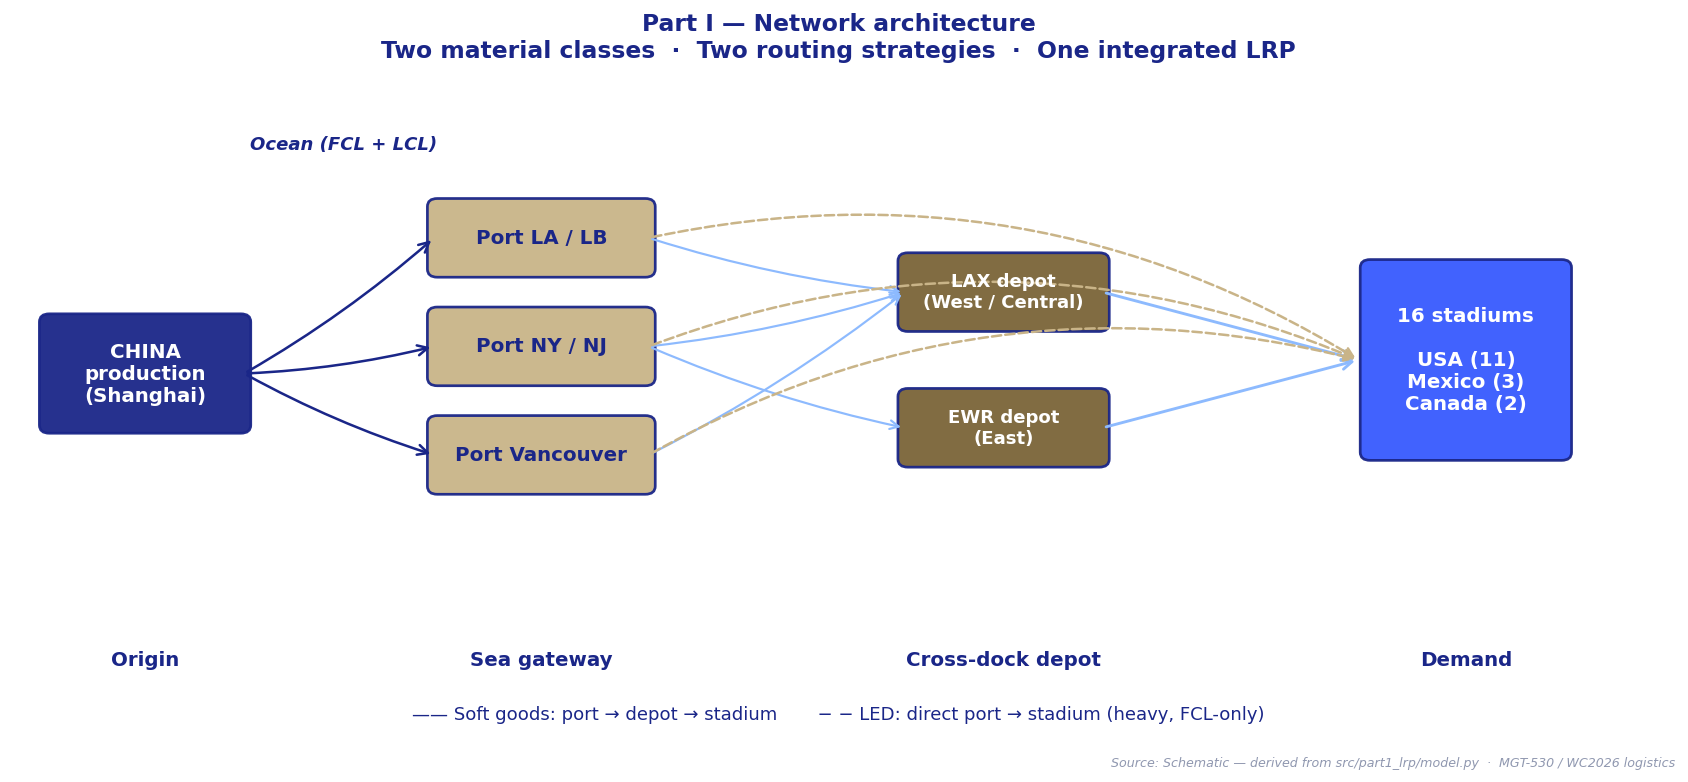
\includegraphics[width=\textwidth]{part1_network_architecture.png}
\caption{Conceptual architecture of the venue-branding supply chain. China is the unique production origin; ocean transport reaches five candidate ports; soft goods are consolidated at depots while LED material flows directly to stadiums.}
\label{fig:architecture}
\end{figure}

\subsection{Scope and contributions}

This report contributes five tangible deliverables:

\begin{enumerate}[leftmargin=*,itemsep=2pt,topsep=2pt]
\item A \textbf{transparent reconstruction} of the WC2026 branding inventory, extrapolated from publicly-available Qatar 2022 data and 11 documented assumptions (Sections~\ref{sec:data} and Appendix~\ref{app:reconstruction}).
\item A \textbf{deterministic Location-Routing Problem} formulation incorporating a \emph{multidimensional} container constraint (volume \emph{and} weight), which produces a 71-vs-40 FEU gap relative to volume-only models (Section~\ref{sec:partI}).
\item A \textbf{Plackett-Luce scenario generator} that produces 50 internally-consistent R32 bracket realisations from publicly-available team-strength priors (Sections~\ref{sec:data},~\ref{sec:partII}).
\item A \textbf{two-stage stochastic MILP} solved as a single deterministic-equivalent program, identifying the matches that cannot feasibly be served reactively and must be pre-positioned (Section~\ref{sec:partII}).
\item Three concrete \textbf{managerial recommendations} grounded in the model outputs, each tied to a sensitivity analysis demonstrating its robustness (Section~\ref{sec:recommendations}).
\end{enumerate}

\subsection{Document structure}

Section~\ref{sec:data} describes the data foundation: the network CSVs (provided), the demand reconstruction (built from inventory anchors), and the scenario data for Part II. Section~\ref{sec:partI} formulates and solves the deterministic LRP. Section~\ref{sec:partII} formulates and solves the two-stage stochastic program. Section~\ref{sec:recommendations} synthesises managerial insights. Section~\ref{sec:limitations} acknowledges limitations and outlines extensions. Appendices~\ref{app:reconstruction}--\ref{app:reproducibility} provide the supporting detail (reconstruction methodology, assumptions registry, data dictionary, full sensitivity tables, sources, and reproducibility instructions).

%==============================================================================
%  SECTION 2 — DATA FOUNDATIONS
%==============================================================================
\section{Data foundations}\label{sec:data}

The data pipeline rests on three layers: the physical network (provided as raw CSVs by a team member), the per-stadium demand (\emph{reconstructed} from inventory anchors because per-venue figures are not publicly available), and the scenario data for the Round of 32 (generated by Monte-Carlo simulation). This section summarises the three layers; full methodological detail is in Appendices~\ref{app:reconstruction} and~\ref{app:datadict}.

\subsection{Network data}\label{sec:data:network}

A team member compiled the network description from FIFA's published venue list \cite{fifa2026official}, U.S./Canadian/Mexican port directories, and publicly-available depot cost benchmarks. \Cref{tab:network} summarises the six CSV files in \filename{data/raw/}; the full schema appears in Appendix~\ref{app:datadict}.

\begin{table}[h]
\centering
\small
\caption{Raw network CSVs (\filename{data/raw/}).}
\label{tab:network}
\begin{tabular}{@{}lrl@{}}
\toprule
\textbf{File} & \textbf{Rows} & \textbf{Content} \\
\midrule
\filename{nodes.csv} & 35 & Master list of all physical locations (lat/lon, type) \\
\filename{ports.csv} & 6 (5 usable) & Ocean-port gateways with FCL/LCL/customs/handling rates \\
\filename{depots.csv} & 7 & Candidate cross-dock depots with fixed and handling costs \\
\filename{stadiums.csv} & 16 & Host stadiums with capacity, city, country, cluster \\
\filename{production\_sites.csv} & 6 & Material producers (The Look Company \& Wasserman Live + China) \\
\filename{storage\_scenarios.csv} & 3 & Low/base/high storage cost scenarios for Part II \\
\filename{edges.csv} & 524 & Sea (5) and road (519) transport links with cost, distance, transit \\
\bottomrule
\end{tabular}
\end{table}

Two pragmatic exclusions are worth flagging: the port of Veracruz appears in \filename{ports.csv} but lacks an FCL rate and is therefore excluded (no maritime cost can be assigned); the port of Manzanillo has no published LCL rate and is therefore included in FCL flows only. These two facts reduce the active port set from six to four for FCL flows and from five to four for LCL flows.

\subsection{Demand reconstruction}\label{sec:data:demand}

\paragraph{Why reconstruction is necessary.} The project CSVs provide the network and all cost parameters but not the per-stadium demand: the file \filename{inventory\_template.csv} referenced in the original project description is missing. We therefore reconstructed per-stadium demand from public anchors: The Look Company's aggregate figure of 905{,}000~\msq{} for Qatar 2022 \cite{thelookcompany_qatar}, bluemedia's $\sim$9{,}300~\msq{} per-stadium building-wrap ratio for Super Bowl LIII \cite{bluemedia_superbowl}, CSM Live's $\sim$3{,}000~\msq{} seat-cover benchmark \cite{csmlive_dressing}, and JYVISIONS' one-FEU-per-stadium LED perimeter specification \cite{jyvisions_led}.

\paragraph{Three ventilation keys.} The reconstructed inventory was apportioned to stadiums through three physically-motivated keys, applied per \emph{poste} (equipment category):

\begin{itemize}[leftmargin=*,itemsep=2pt,topsep=2pt]
\item \textbf{Capacity key} (interior, seat covers, building wraps, vehicle wraps). The poste volume is allocated proportionally to seating capacity: $V_{p,s} = V_p \cdot \mathrm{cap}_s / \sum_{s'} \mathrm{cap}_{s'}$.
\item \textbf{Fixed key} (LED perimeter, pitch-side, wayfinding, alu totems, masts, fence scrim). The poste volume is split equally across the 16 stadiums: $V_{p,s} = V_p / 16$. This applies to items whose physical specification is venue-independent (one LED system per stadium, one 105~$\times$~68~m pitch perimeter, etc.).
\item \textbf{Typology key} (brand scrubbing only — the 2026-specific poste). Stadiums are clustered into three tiers reflecting the intensity of pre-existing permanent branding to mask: 8 heavily-branded NFL venues at $\sim$6{,}000~\msq{} each, 5 recent venues at $\sim$3{,}000~\msq{}, and 3 Mexican/Canadian venues at $\sim$2{,}100~\msq{} \cite{sbj_facilitiesdive}.
\end{itemize}

\paragraph{Reconciliation.} Summing across postes and stadiums reconciles \emph{exactly} to the Qatar-to-2026 extrapolated totals: \textbf{2{,}726.0~\mcube{} and 1{,}828.0~\tonne{}}, of which 1{,}072~\mcube{} are LED (heavy, $\rho \approx 0.99$~\tonne/\mcube) and 1{,}654~\mcube{} are soft goods (light, $\rho \approx 0.46$~\tonne/\mcube). \Cref{fig:stad-demand} shows the per-stadium decomposition.

\begin{figure}[H]
\centering
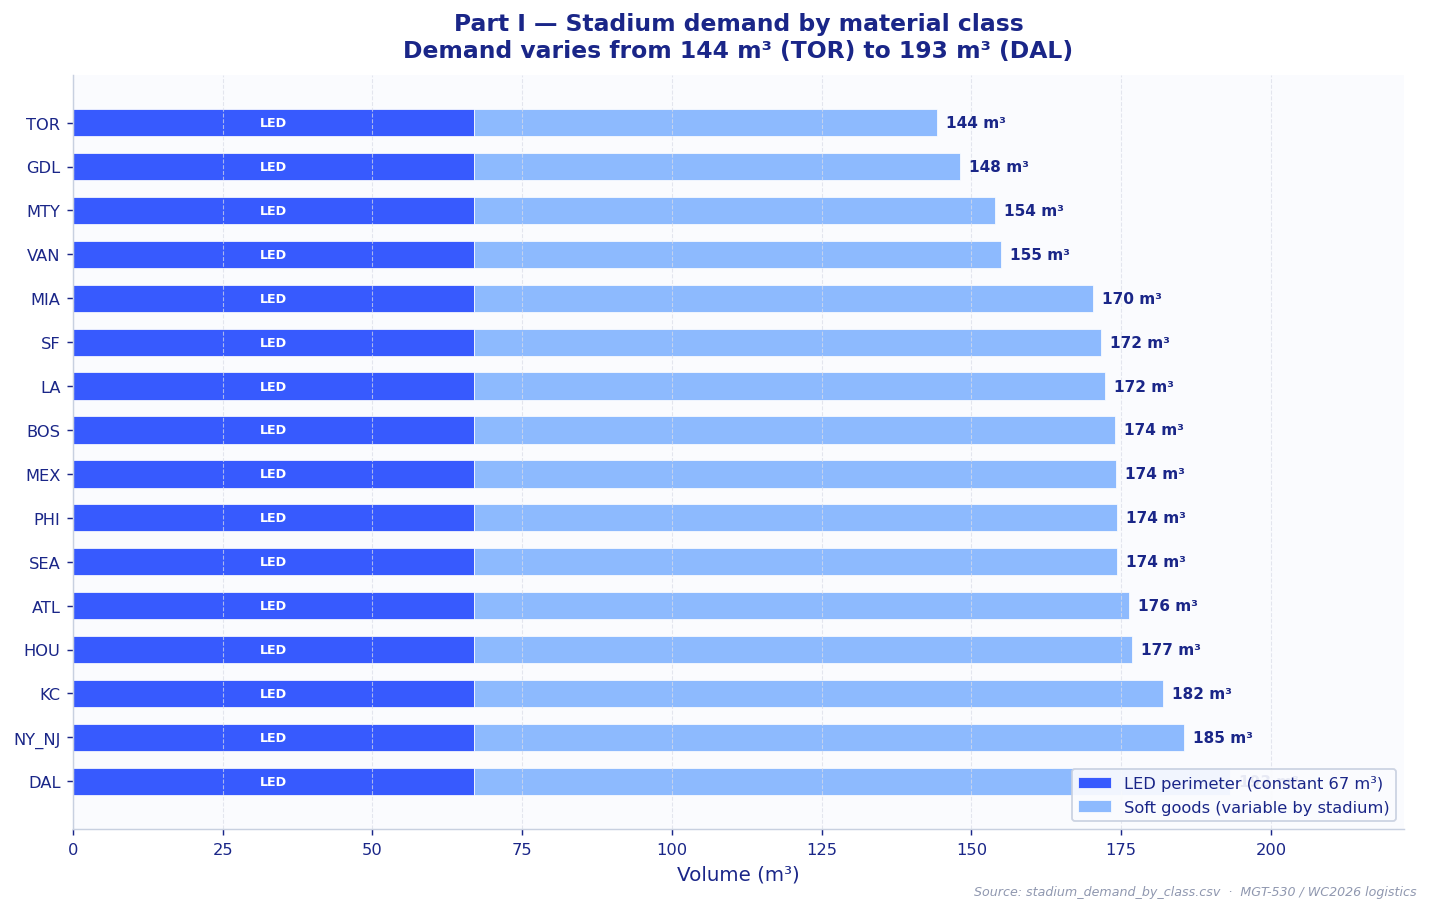
\includegraphics[width=\textwidth]{part1_stadium_demand.png}
\caption{Reconstructed demand per stadium, decomposed into LED (constant 67~\mcube{} per stadium, blue) and soft goods (variable, light blue). Dallas hosts the largest demand (193~\mcube{}), Toronto the smallest (144~\mcube{}).}
\label{fig:stad-demand}
\end{figure}

\subsection{Key physical and cost parameters}\label{sec:data:parameters}

\Cref{tab:params} summarises the parameters that appear in both models, classified by sourcing status: \statusSourced{} externally sourced (peer-reviewed or industry-standard), \statusDerived{} derived from project data or simple arithmetic, and \statusAssumed{} assumed-with-sensitivity (covered by explicit ranges in Section~\ref{sec:partI:sensitivity} and~\ref{sec:partII:sensitivity}). The full registry of 20 assumptions appears in Appendix~\ref{app:assumptions}.

\begin{table}[h]
\centering
\small
\caption{Key physical and cost parameters. Status: \statusSourced{} sourced, \statusDerived{} derived, \statusAssumed{} assumed with sensitivity range.}
\label{tab:params}
\begin{tabularx}{\textwidth}{@{}l l c X@{}}
\toprule
\textbf{Symbol} & \textbf{Value} & \textbf{Status} & \textbf{Source / Derivation} \\
\midrule
$\mathrm{FEU}$ & 67~\mcube{} & \statusSourced{} & ISO 668 40-ft container interior volume \cite{iso_container} \\
$\mathrm{PAY}$ & 26~\tonne{} & \statusSourced{} & U.S. road weight limit; ISO gross 30.48~\tonne{} minus 3.7~\tonne{} tare \cite{fmcsa_weight} \\
$\mathrm{TRUCK}$ & 90~\mcube{} & \statusSourced{} & U.S. dry-van trailer usable volume \\
$\rho_{\mathrm{LED}}$ & 0.994~\tonne/\mcube & \statusDerived{} & 1{,}066~\tonne / 1{,}072~\mcube{} from inventory \\
$\rho_{\mathrm{SOFT}}$ & 0.46~\tonne/\mcube & \statusDerived{} & 762~\tonne / 1{,}654~\mcube{} from inventory \\
Production cost & \USD{50}/\msq{} & \statusSourced{} & 2026 U.S. large-format market \cite{costhack_printing} \\
Rush lead time & 1~day & \statusSourced{} & Industry same-day printing \cite{signsnyc_rush} \\
Storage cost & \USD{0.03}/\USD{0.08}/\USD{0.15} per \mcube/day & \statusAssumed{} & FIFA depot cost not public; low/base/high sensitivity \\
Anticipatory waste factor & $2\times$ & \statusAssumed{} & Cover two candidate teams; 1$\times$/2$\times$/3$\times$ sensitivity \\
Production fill rate & 57\% & \statusDerived{} & Rouleau geometry plus realistic voids \\
\bottomrule
\end{tabularx}
\end{table}

\subsection{Stochastic data for Part~II}\label{sec:data:scenarios}

The Round-of-32 bracket is partially deterministic and partially stochastic. \emph{Venues} and \emph{dates} are fixed (publicly scheduled at the time of writing), but \emph{team identities} are uncertain until the group stage finishes on 27 June 2026 and the bracket fills.

\paragraph{Strength prior.} We extract team-strength priors from publicly-available tournament-winner odds (user-collected bookmaker screenshots, May 2026), normalised to remove the bookmaker margin: $\sigma_t = (1/o_t) / \sum_{t'} (1/o_{t'})$. The resulting strength ordering matches the Opta supercomputer \cite{opta_supercomputer} to within rounding (Spain $\approx$16.5\%, France $\approx$15\%, England $\approx$11\%), giving us confidence in the prior as a strength proxy.

\paragraph{Scenario generation.} For each of 50 Monte-Carlo runs we (i) simulate the 12 group stages by drawing rankings using a strength-weighted Plackett-Luce model \cite{plackett1975}, (ii) collect the 12 third-placed teams and assign the eight strongest to the bracket's third-slot positions respecting allowed-group constraints, (iii) propagate teams through the fixed bracket structure to obtain a complete 16-match R32 realisation. Each scenario receives probability $1/50$.

\Cref{fig:timeline} illustrates the two-stage decision structure that this scenario data drives. The Stage-1 decision (anticipatory pre-positioning) is taken \emph{before} any scenario is realised; the Stage-2 decision (reactive production and trucking) is taken \emph{per scenario} after the draw.

\begin{figure}[H]
\centering
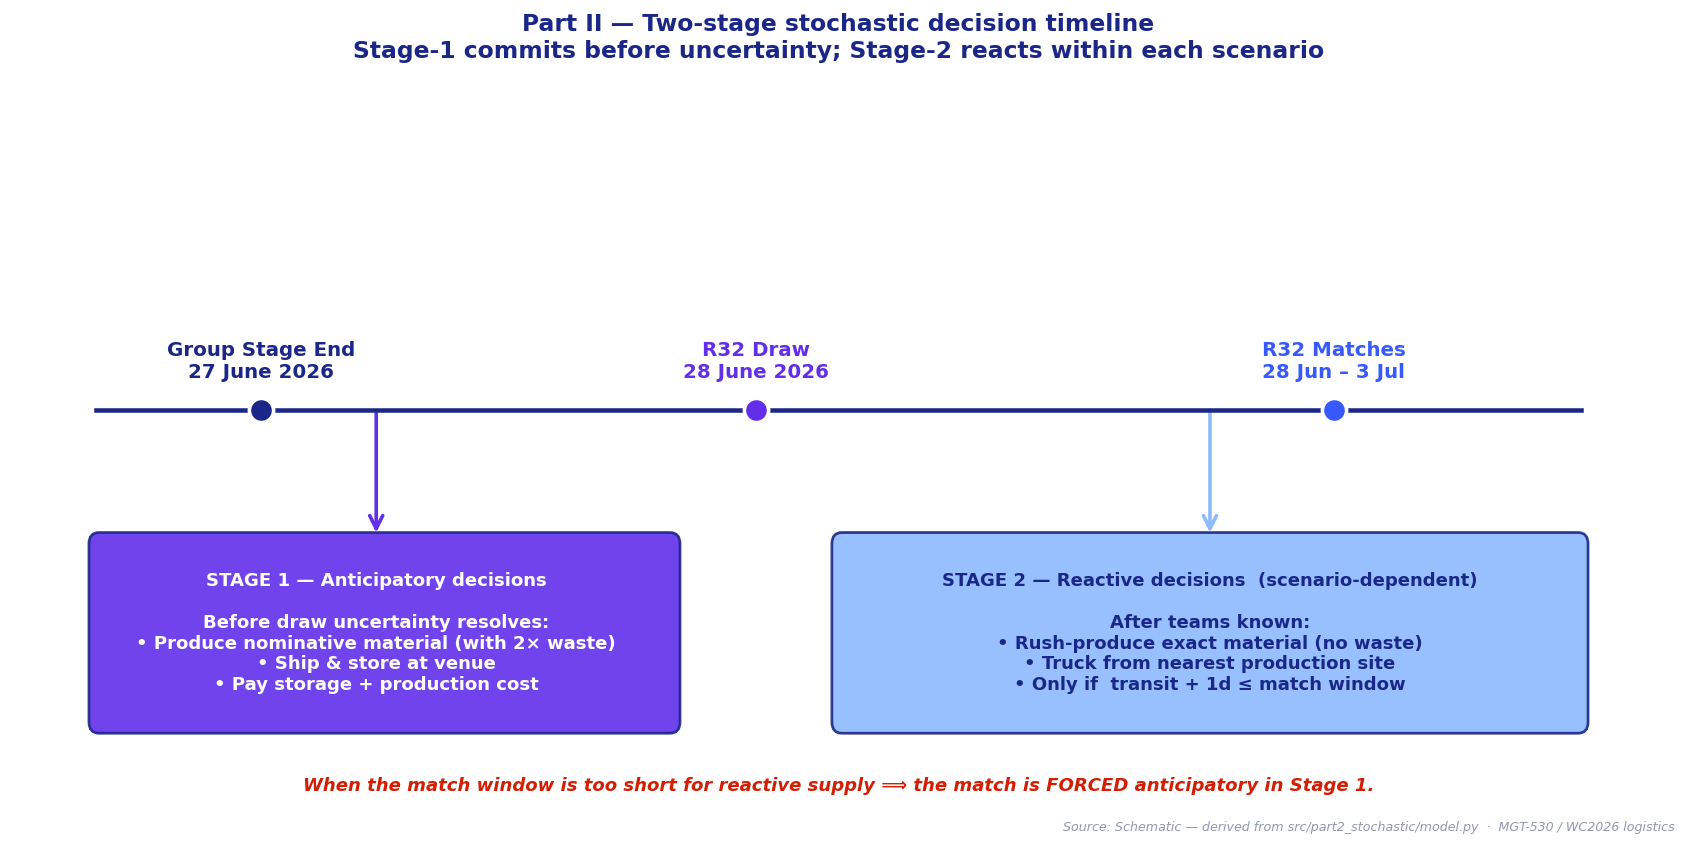
\includegraphics[width=\textwidth]{part2_two_stage_timeline.png}
\caption{Two-stage stochastic decision timeline. Stage-1 commits anticipatory production and storage before the R32 draw; Stage-2 reacts within each realised scenario, but only for matches whose time window admits reactive supply.}
\label{fig:timeline}
\end{figure}

%==============================================================================
%  SECTION 3 — PART I LRP
%==============================================================================
\section{Part~I — Deterministic Location-Routing Problem}\label{sec:partI}

\subsection{Problem statement}

For the generic branding stream we formulate a single integrated Mixed-Integer Linear Program (MILP) that decides simultaneously which sea-port gateways to open, which cross-dock depots to open, and how to route every cubic metre of demand from ports to depots and from depots (or, for LED, directly) to stadiums. The model is a classical Location-Routing Problem in the sense of Daskin \cite{daskin_location}, augmented with a \emph{multidimensional} container-capacity constraint that distinguishes our formulation from textbook examples.

\paragraph{Two material classes with opposite physics.} The branding inventory contains two flow classes that behave oppositely in containers:

\begin{itemize}[leftmargin=*,itemsep=3pt,topsep=2pt]
\item \textbf{LED} (perimeter boards, $\rho \approx 0.99$~\tonne/\mcube). Dense and rigid; ships exclusively as Full Container Load (FCL) and goes directly from the port to each stadium, bypassing depots (oversized and fragile, one system per stadium \cite{jyvisions_led}). For LED the binding container constraint is \emph{weight}, not volume.
\item \textbf{Soft goods} (vinyl, mesh, fabric; $\rho \approx 0.46$~\tonne/\mcube). Lighter and consolidatable; can ship FCL or as Less-than-Container-Load (LCL); flows port $\rightarrow$ depot $\rightarrow$ stadium. For soft goods the binding constraint is \emph{volume}.
\end{itemize}

This two-class structure motivates a separate FEU count per class, per port, and is the mechanism by which the model reproduces a non-trivial 71-vs-40 FEU gap. Before formulating the model, \Cref{fig:feu-box} gives the geometric intuition.

\begin{figure}[H]
\centering
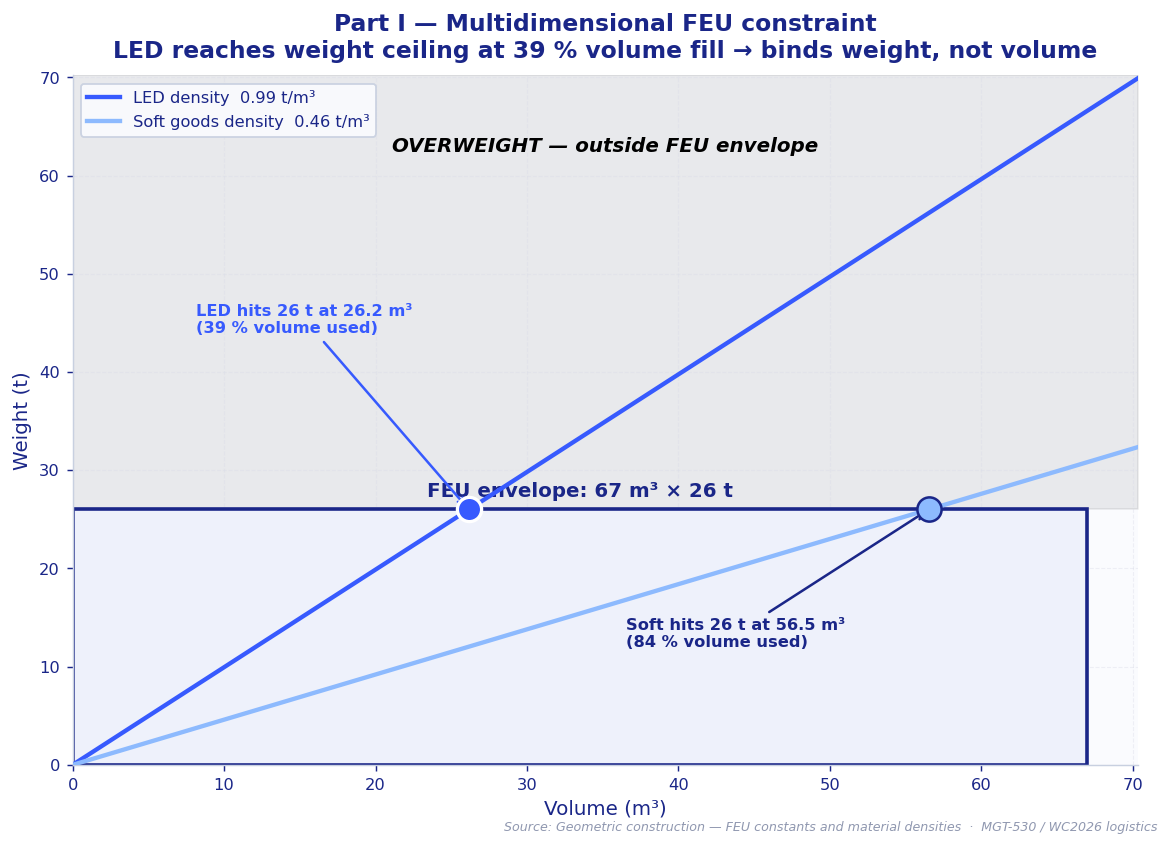
\includegraphics[width=0.85\textwidth]{part1_feu_constraint_box.png}
\caption{Geometric view of the multidimensional FEU constraint. The dark-blue ray traces LED at its density of 0.99~\tonne/\mcube{}: it strikes the 26~\tonne{} payload ceiling at 26.2~\mcube — only 39\% of the 67~\mcube{} volume. Soft goods strike the same ceiling at 56.5~\mcube{} (84\% volume).}
\label{fig:feu-box}
\end{figure}

\subsection{Mathematical formulation}\label{sec:partI:model}

\paragraph{Sets and indices.}
\[
\mathcal{S}\ \text{(stadiums, $|\mathcal{S}| = 16$)},\quad
\mathcal{P}\ \text{(ports, $|\mathcal{P}| = 5$)},\quad
\mathcal{D}\ \text{(depots, $|\mathcal{D}| = 7$)}.
\]

\paragraph{Parameters.} See \Cref{tab:params} for the headline physical constants. Cost parameters per port $p \in \mathcal{P}$ are FCL rate $\mathrm{fcl}_p$, LCL rate $\mathrm{lcl}_p$, customs $\mathrm{cus}_p$ and handling $\mathrm{hnd}_p$ (per FEU); per depot $d \in \mathcal{D}$ are fixed cost $\mathrm{fix}_d$ and handling-per-volume cost $\mathrm{hnd}^{\mathcal{D}}_d$. Trucking cost per truck on arc $a$ is $\mathrm{tc}_a = \mathrm{km}_a \cdot \mathrm{cpk}_a + \mathrm{bcost}_a$ (with $\mathrm{bcost}$ adding a border-crossing premium where applicable). The demand per stadium is split into two classes: $V^{\mathrm{led}}_s$ and $V^{\mathrm{soft}}_s$.

\paragraph{Decision variables.} \Cref{tab:partI-vars} catalogues all variables.

\begin{table}[h]
\centering
\small
\caption{Part~I decision variables.}
\label{tab:partI-vars}
\begin{tabular}{@{}l l l@{}}
\toprule
\textbf{Variable} & \textbf{Type} & \textbf{Meaning} \\
\midrule
$o_p \in \{0,1\}$        & binary     & port $p$ is opened \\
$o_d \in \{0,1\}$        & binary     & depot $d$ is opened \\
$n^{\mathrm{led}}_p \in \mathbb{Z}_+$ & integer & FEUs of LED material loaded at port $p$ \\
$n^{\mathrm{soft}}_p \in \mathbb{Z}_+$ & integer & FEUs of soft goods loaded at port $p$ \\
$\ell_p \ge 0$            & continuous & LCL volume of soft goods at port $p$ (\mcube) \\
$x^{\mathrm{soft}}_{p,d} \ge 0$ & continuous & Soft goods flow port $p$ $\to$ depot $d$ (\mcube) \\
$y^{\mathrm{soft}}_{d,s} \ge 0$ & continuous & Soft goods flow depot $d$ $\to$ stadium $s$ (\mcube) \\
$x^{\mathrm{led}}_{p,s} \ge 0$ & continuous & LED direct flow port $p$ $\to$ stadium $s$ (\mcube) \\
$t^{\mathrm{pd}}_{p,d}, t^{\mathrm{ds}}_{d,s}, t^{\mathrm{ps}}_{p,s} \in \mathbb{Z}_+$ & integer & Whole-truck counts on each road arc type \\
\bottomrule
\end{tabular}
\end{table}

\paragraph{Objective.} Minimise the sum of ocean costs (FCL + LCL + opening customs + per-FEU handling), depot opening fixed costs, depot per-volume handling, and three types of whole-truck trucking:
\begin{align}
\min\ Z\ =\ &\ \sum_{p\in\mathcal{P}} \!\Big[(n^{\mathrm{led}}_p + n^{\mathrm{soft}}_p)(\mathrm{fcl}_p + \mathrm{hnd}_p) + o_p\, \mathrm{cus}_p + \ell_p\, \mathrm{lcl}_p\Big]\nonumber\\
&\ + \sum_{d\in\mathcal{D}} o_d\, \mathrm{fix}_d
\ +\ \sum_{d\in\mathcal{D}}\!\Big(\sum_{s\in\mathcal{S}} y^{\mathrm{soft}}_{d,s}\Big)\, \mathrm{hnd}^{\mathcal{D}}_d\nonumber\\
&\ + \sum_{(p,d)} t^{\mathrm{pd}}_{p,d}\, \mathrm{tc}_{p,d}
\ +\ \sum_{(d,s)} t^{\mathrm{ds}}_{d,s}\, \mathrm{tc}_{d,s}
\ +\ \sum_{(p,s)} t^{\mathrm{ps}}_{p,s}\, \mathrm{tc}_{p,s}.\label{eq:partI-obj}
\end{align}

\paragraph{Constraints.} We group them into five blocks. Equations \eqref{eq:partI-C1a}--\eqref{eq:partI-C5} are the complete model.

\textit{(C1) Demand satisfaction (per class, per stadium).}
\begin{align}
\sum_{d \in \mathcal{D}} y^{\mathrm{soft}}_{d,s} &= V^{\mathrm{soft}}_s &&\forall s \in \mathcal{S}, \label{eq:partI-C1a}\\
\sum_{p \in \mathcal{P}} x^{\mathrm{led}}_{p,s} &= V^{\mathrm{led}}_s &&\forall s \in \mathcal{S}. \label{eq:partI-C1b}
\end{align}

\textit{(C2) Flow conservation at each depot} — inflow equals outflow (soft only; LED bypasses depots):
\begin{equation}
\sum_{p \in \mathcal{P}} x^{\mathrm{soft}}_{p,d} = \sum_{s \in \mathcal{S}} y^{\mathrm{soft}}_{d,s} \qquad \forall d \in \mathcal{D}. \label{eq:partI-C2}
\end{equation}

\textit{(C3) Multidimensional sea capacity per port} — both volume and weight must fit:
\begin{align}
\sum_{d \in \mathcal{D}} x^{\mathrm{soft}}_{p,d} &\le \mathrm{FEU}\cdot n^{\mathrm{soft}}_p + \ell_p && \forall p \in \mathcal{P}, \label{eq:partI-C3a}\\
\rho_{\mathrm{SOFT}}\!\sum_{d \in \mathcal{D}} x^{\mathrm{soft}}_{p,d} &\le \mathrm{PAY}\cdot n^{\mathrm{soft}}_p + \rho_{\mathrm{SOFT}}\,\ell_p && \forall p \in \mathcal{P}, \label{eq:partI-C3b}\\
\sum_{s \in \mathcal{S}} x^{\mathrm{led}}_{p,s} &\le \mathrm{FEU}\cdot n^{\mathrm{led}}_p && \forall p \in \mathcal{P}, \label{eq:partI-C3c}\\
\rho_{\mathrm{LED}}\!\sum_{s \in \mathcal{S}} x^{\mathrm{led}}_{p,s} &\le \mathrm{PAY}\cdot n^{\mathrm{led}}_p && \forall p \in \mathcal{P}. \label{eq:partI-C3d}
\end{align}

\textit{(C4) Big-M opening coupling} — no FEU at a port and no flow out of a depot unless the facility is opened (with $M = \sum_s (V^{\mathrm{soft}}_s + V^{\mathrm{led}}_s)$):
\begin{align}
n^{\mathrm{soft}}_p,\ n^{\mathrm{led}}_p &\le \Big(\tfrac{M}{\mathrm{FEU}}+1\Big)\, o_p, \quad \ell_p \le M\, o_p && \forall p \in \mathcal{P},\label{eq:partI-C4a}\\
\sum_{s \in \mathcal{S}} y^{\mathrm{soft}}_{d,s} &\le M\, o_d && \forall d \in \mathcal{D}.\label{eq:partI-C4b}
\end{align}

\textit{(C5) Whole-truck packing} — every road arc carries integer trucks:
\begin{equation}
\mathrm{TRUCK} \cdot t^{a}_{u,v} \ \ge \ \text{(volume on arc $a$ between $u$ and $v$)} \quad \forall\,(u,v,a). \label{eq:partI-C5}
\end{equation}

\begin{keybox}
The model's distinguishing feature is the \emph{multidimensional} sea-capacity block (C3), which enforces both volume \eqref{eq:partI-C3a},\eqref{eq:partI-C3c} and weight \eqref{eq:partI-C3b},\eqref{eq:partI-C3d} ceilings per FEU. For LED, weight binds first: 26~\tonne{} is reached at 26.2~\mcube{}, exhausting only 39\% of the 67~\mcube{} volume. The model therefore loads 42 LED FEUs even though the volume content (1{,}072~\mcube) would fit in 16. This is the \emph{LED weight effect} (Section~\ref{sec:partI:setup}).
\end{keybox}

\subsection{Baseline results}\label{sec:partI:baseline}

The model solves to optimality in well under one second using SCIP \cite{scip} via OR-Tools \cite{ortools}. \Cref{tab:partI-baseline} summarises the headline numbers; \Cref{fig:network-map} shows the resulting network on a map of North America.

\begin{table}[h]
\centering
\small
\caption{Part~I baseline optimal solution (LED direct, depots, weight constraint enforced, LCL allowed).}
\label{tab:partI-baseline}
\begin{tabular}{@{}lr@{}}
\toprule
\textbf{Quantity} & \textbf{Value} \\
\midrule
Total cost & \USD{458{,}626} \\
Total FEUs & 71 \\
\quad LED FEUs & 42 \\
\quad Soft-goods FEUs & 29 \\
Open ports & LA/Long Beach, New York/NJ, Vancouver \\
Open depots & LAX (West/Central), EWR (East) \\
Ocean freight share & 68.0\% \\
Depot fixed + handling share & 12.5\% \\
Trucking (all arcs) share & 19.7\% \\
\bottomrule
\end{tabular}
\end{table}

\begin{figure}[H]
\centering
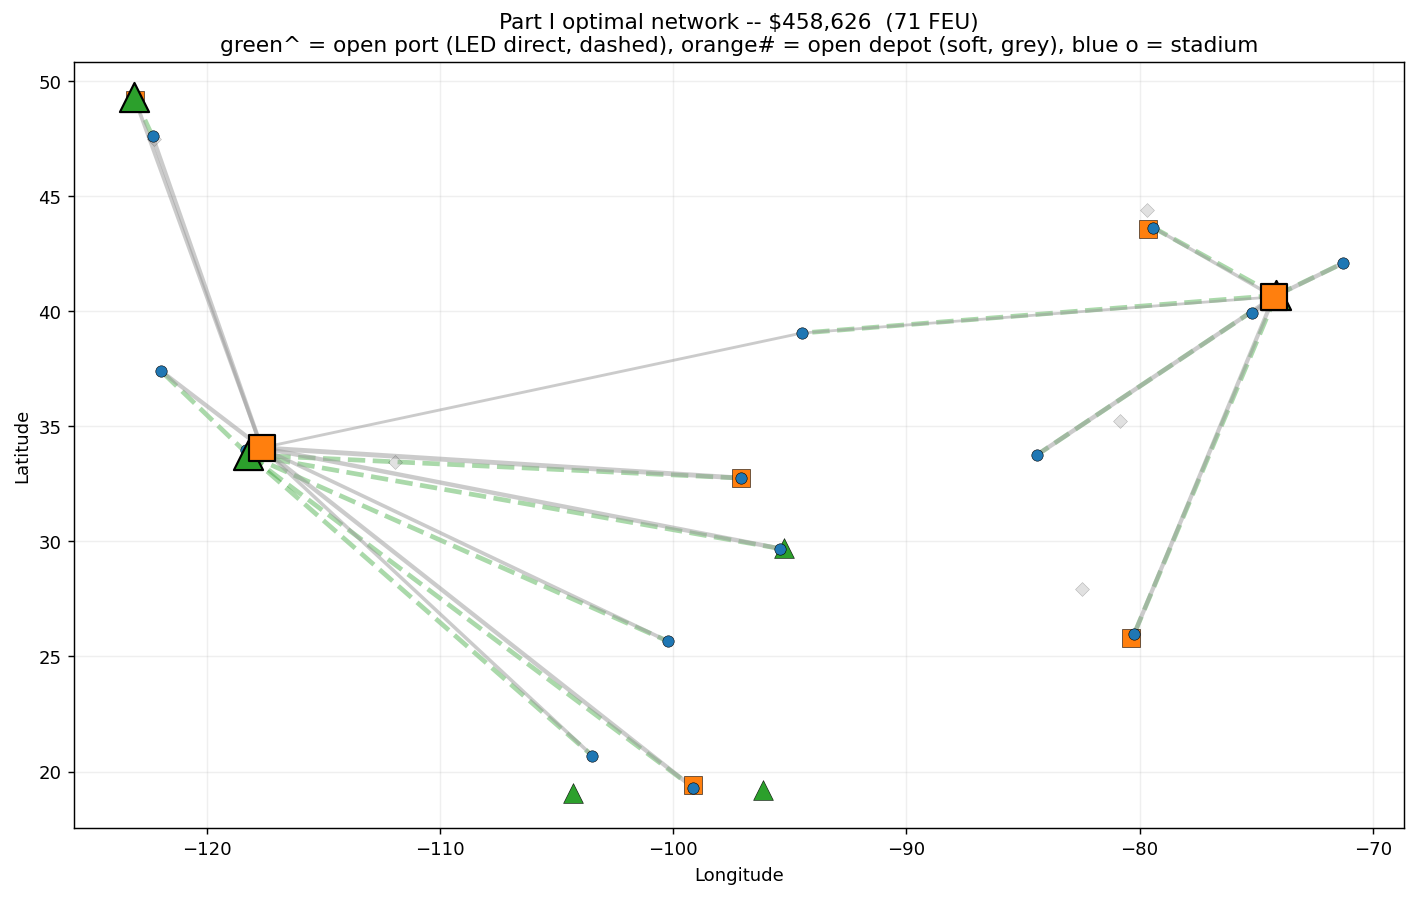
\includegraphics[width=\textwidth]{part1_network_map.png}
\caption{Optimal Part~I network on a North-American backdrop. Three sea-port gateways (LA, NY, VAN) feed two cross-dock depots (LAX, EWR). Soft-goods flows (blue lines) move via depots; LED flows (dashed lime) move directly to each stadium.}
\label{fig:network-map}
\end{figure}

The cost composition is unbalanced: ocean freight alone accounts for two-thirds of the total (\Cref{fig:donut}). Practically, this means that any optimisation lever that does not target ocean freight will have limited overall impact.

\begin{figure}[H]
\centering
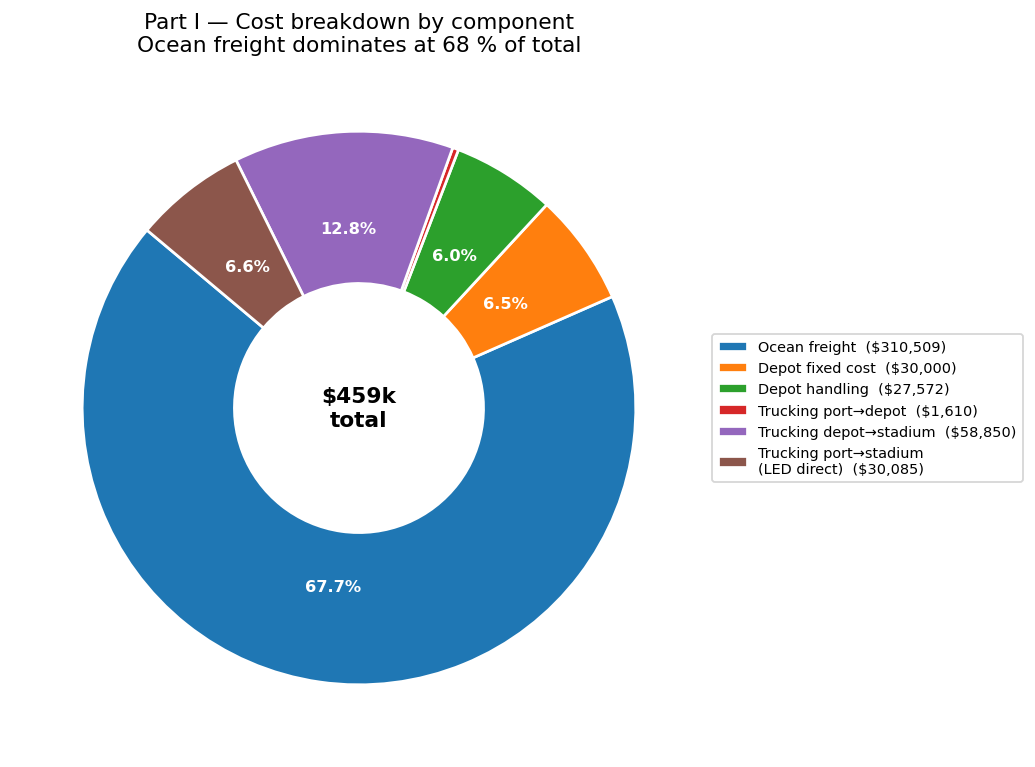
\includegraphics[width=0.8\textwidth]{part1_cost_donut.png}
\caption{Cost breakdown by component. Ocean freight ($\sim$\USD{310k}) is the dominant lever; depot-to-stadium trucking is the second-largest item (\USD{59k}, 12.8\%).}
\label{fig:donut}
\end{figure}

\subsection{Configuration comparison and the LED weight effect}\label{sec:partI:setup}

To isolate \emph{which model features drive the result}, we re-solved the LRP under four contrasted setups: the baseline, an alternative routing LED via depots, a configuration that ignores the weight constraint (volume-only), and an FCL-only configuration (LCL disabled). \Cref{tab:setups} compares them.

\begin{table}[h]
\centering
\small
\caption{Setup comparison. The volume-only configuration is non-physical (containers would overweight at port) but quantifies the magnitude of the LED weight effect.}
\label{tab:setups}
\begin{tabular}{@{}lrrrr@{}}
\toprule
\textbf{Setup} & \textbf{Total cost} & \textbf{LED FEU} & \textbf{Soft FEU} & \textbf{Total FEU} \\
\midrule
Baseline (LED direct, weight, LCL) & \USD{458{,}626} & 42 & 29 & 71 \\
LED via depot (no direct route)    & \USD{442{,}760} & 41 & 29 & 70 \\
Volume-only (no weight constraint) & \USD{324{,}180} & 16 & 24 & 40 \\
FCL-only (LCL disabled)            & \USD{461{,}269} & 42 & 30 & 72 \\
\bottomrule
\end{tabular}
\end{table}

\Cref{fig:setup} visualises the same comparison; \Cref{fig:feu-eff} shows the underlying physical reason — LED density saturates the weight ceiling far below the volume ceiling.

\begin{figure}[H]
\centering
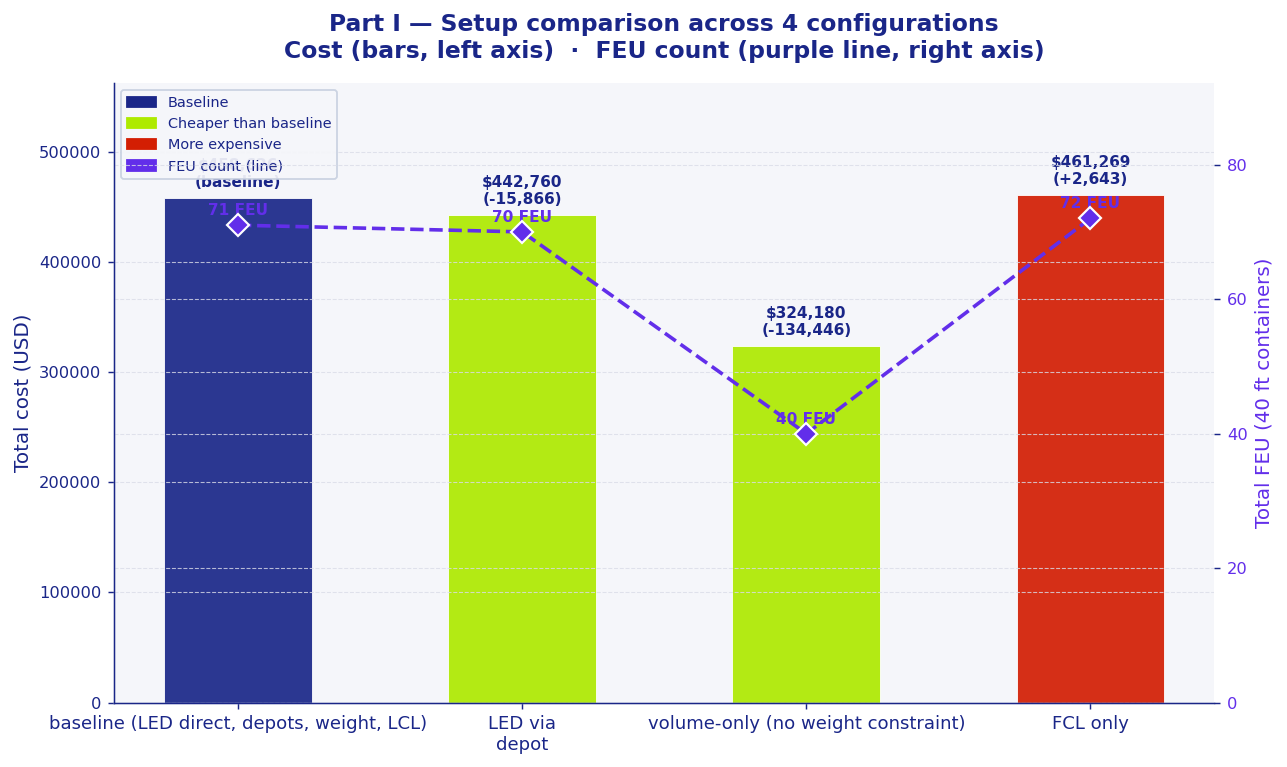
\includegraphics[width=\textwidth]{part1_setup_comparison.png}
\caption{Setup comparison. Cost (bars, left axis) and total FEU count (purple line, right axis). Removing the weight constraint saves \USD{134k} and 31 FEUs, but this is a physically infeasible regime.}
\label{fig:setup}
\end{figure}

\begin{figure}[H]
\centering
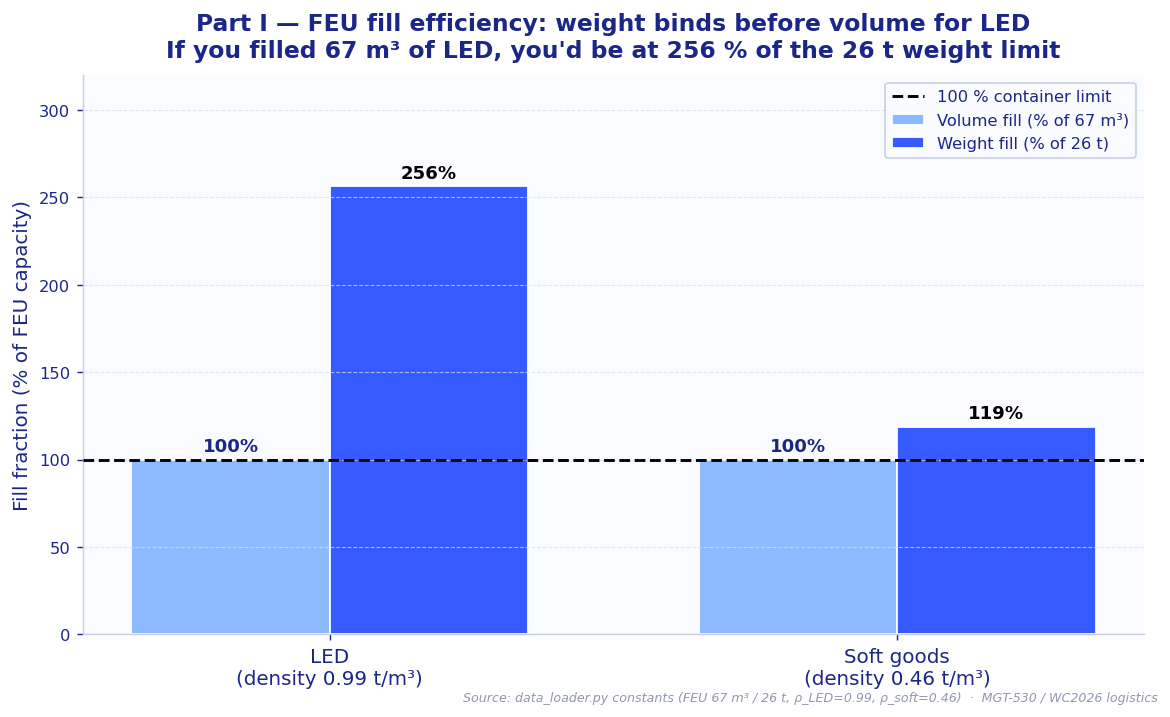
\includegraphics[width=0.78\textwidth]{part1_feu_efficiency.png}
\caption{Container fill efficiency by material class. Filling a FEU with 67~\mcube{} of LED would weigh 256\% of the 26~\tonne{} ceiling — physically impossible. The weight ceiling forces LED to load at only 39\% volume, multiplying the FEU count.}
\label{fig:feu-eff}
\end{figure}

\Cref{fig:feu-class} shows the stacked FEU counts under the two regimes side by side.

\begin{figure}[H]
\centering
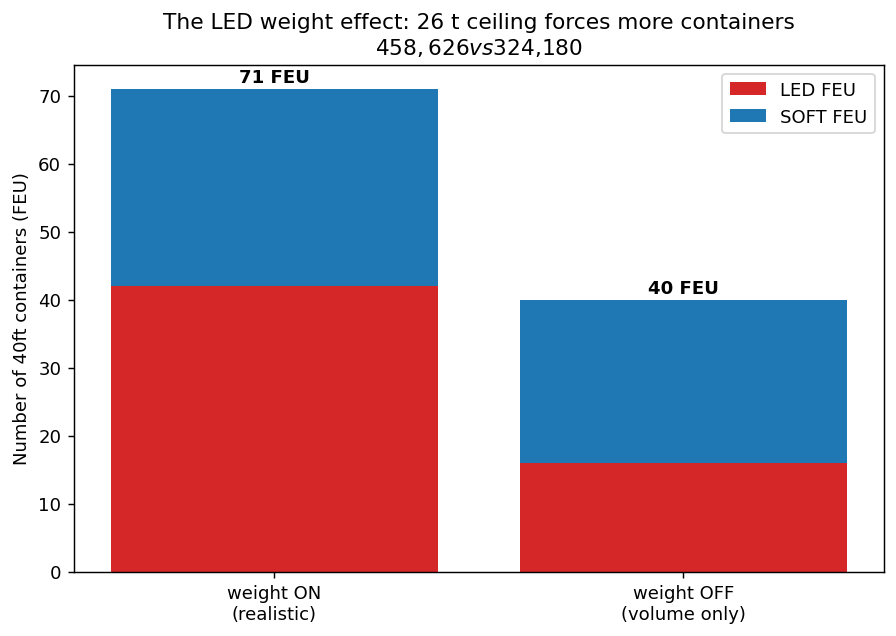
\includegraphics[width=0.75\textwidth]{part1_feu_by_class.png}
\caption{Total FEU count under weight ON vs OFF, decomposed by class. The 31-FEU gap is entirely on the LED side: 42 (weight-driven) vs 16 (volume-only).}
\label{fig:feu-class}
\end{figure}

\subsection{Sensitivity analysis}\label{sec:partI:sensitivity}

We probed three parameters one at a time around the baseline: the weight constraint (on/off), the LED routing strategy (direct/via-depot), and the LCL policy (allowed/FCL-only). \Cref{tab:partI-sens} summarises the sweep and \Cref{fig:partI-tornado} visualises the impact magnitudes.

\begin{table}[h]
\centering
\small
\caption{Part~I one-at-a-time (OAT) sensitivity around the baseline.}
\label{tab:partI-sens}
\begin{tabular}{@{}llrrl@{}}
\toprule
\textbf{Parameter} & \textbf{Value} & \textbf{Total cost} & \textbf{FEU} & \textbf{Open ports} \\
\midrule
weight constraint & on (baseline)    & \USD{458{,}626} & 71 & LA + NY + VAN \\
weight constraint & off              & \USD{324{,}180} & 40 & LA + NY + HOU + VAN \\
LCL policy        & allowed          & \USD{458{,}626} & 71 & LA + NY + VAN \\
LCL policy        & FCL-only         & \USD{461{,}269} & 72 & LA + NY + VAN \\
LED routing       & direct           & \USD{458{,}626} & 71 & LA + NY + VAN \\
LED routing       & via depot        & \USD{442{,}760} & 70 & LA + NY \\
\bottomrule
\end{tabular}
\end{table}

\begin{figure}[H]
\centering
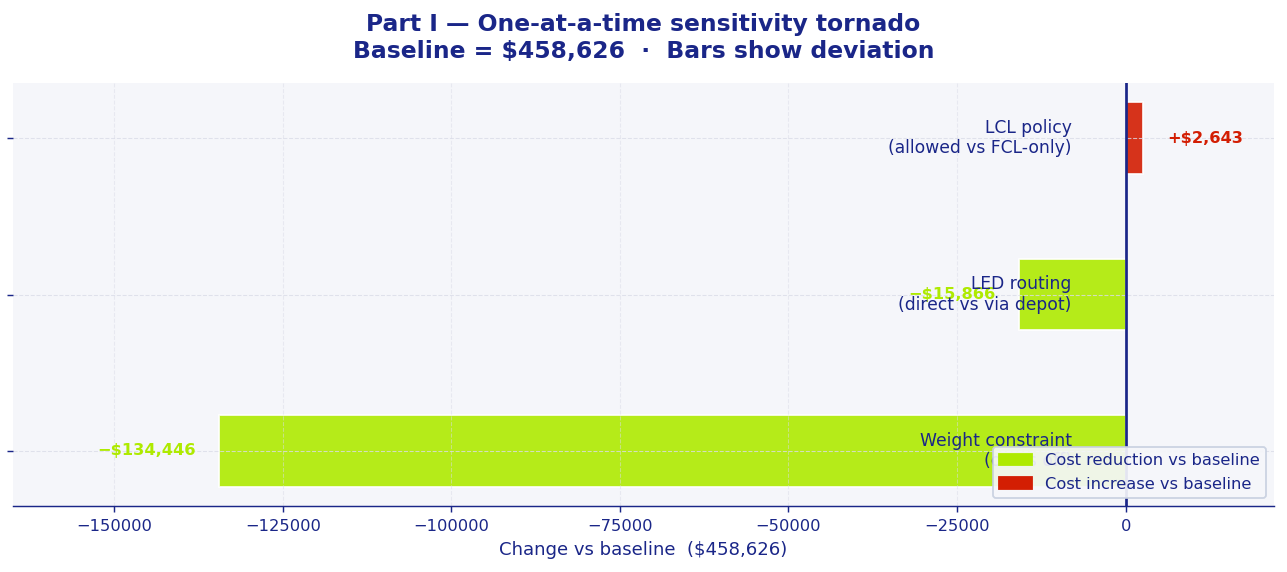
\includegraphics[width=\textwidth]{part1_sensitivity_tornado.png}
\caption{Part~I sensitivity tornado. The weight constraint dominates by an order of magnitude; LCL and LED routing have marginal effects.}
\label{fig:partI-tornado}
\end{figure}

The key managerial takeaway is that \textbf{the only parameter that meaningfully moves total cost is the weight constraint itself}, which is non-negotiable physics. The two design choices (LED routing and LCL) shift cost by 1--4\% only. The model is therefore robust: the result is not sensitive to design choices an analyst could second-guess.

\subsection{Network structure and port-depot specialisation}

\Cref{fig:flow-mat} shows the soft-goods flow from each depot to each stadium. The optimal solution exhibits clean geographic specialisation: LAX serves all West and Central stadiums, EWR serves all East stadiums, and Kansas City is the only split-served venue.

\begin{figure}[H]
\centering
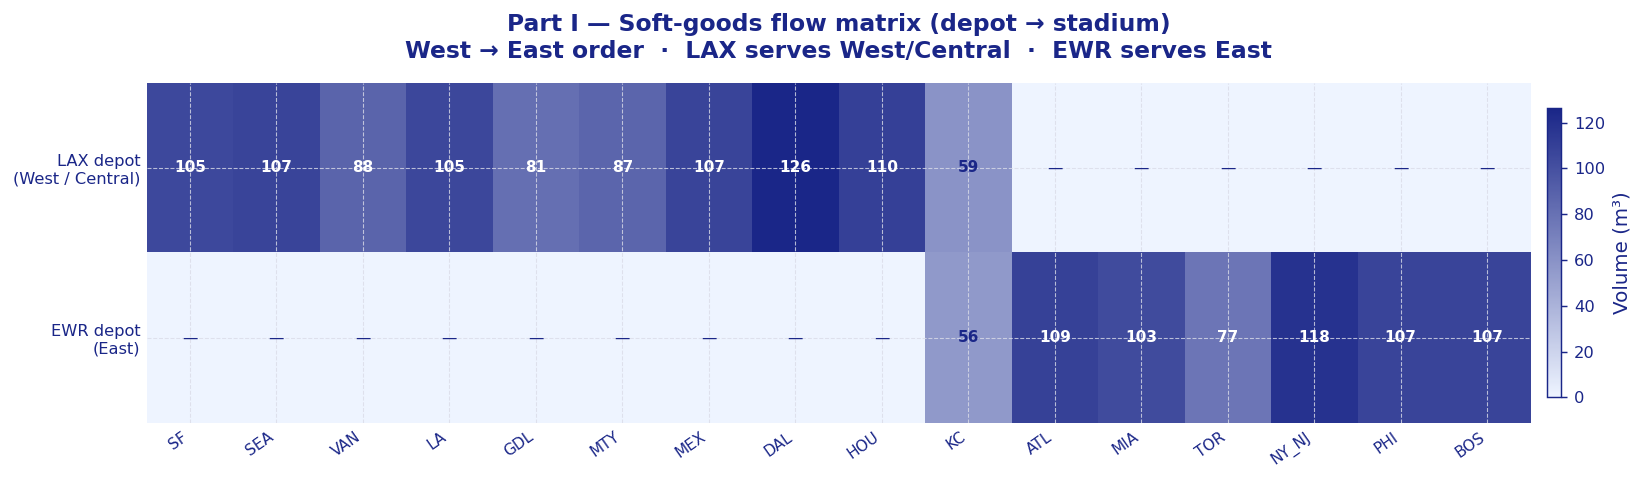
\includegraphics[width=\textwidth]{part1_flow_matrix.png}
\caption{Soft-goods flow matrix (depot $\to$ stadium, \mcube). Order is West $\to$ East. The optimal network partitions cleanly with a small overlap at Kansas City.}
\label{fig:flow-mat}
\end{figure}

Vancouver merits special comment: the port is opened only to receive LED FEUs (6 of them) and ships no soft goods. The port is therefore a \emph{LED-specialist} gateway; closing it would force those 6 LED FEUs through LA, raising West-coast trucking and lengthening the LED transit. The role of Vancouver as a Western-Canadian LED entry point is therefore intrinsic to the optimum, not a coincidence.

%==============================================================================
%  SECTION 4 — PART II STOCHASTIC
%==============================================================================
\section{Part~II — Two-Stage Stochastic Program}\label{sec:partII}

\subsection{Problem statement}

For the nominative material stream we face a fundamentally different problem: only $\sim$6.5~\mcube{} of volume, but its production cannot start until the matchup is known. The Round of 32 begins on 28 June 2026, one day after the group stage ends, leaving a window of 1--6 days per match depending on the date. Whether the material can be produced and trucked in time is a feasibility question, not a cost-minimisation question.

\paragraph{Two supply modes.} We model two production strategies:
\begin{itemize}[leftmargin=*,itemsep=3pt,topsep=2pt]
\item \textbf{Reactive (Stage 2).} After the matchup is known, produce the exact nominative material at a U.S./Canadian print site, then truck it to the venue. Feasible only when $\mathrm{transit}(j \!\to\! v_m) + \mathrm{prod\_days} \le \mathrm{window}(m)$.
\item \textbf{Anticipatory (Stage 1).} Before the matchup is known, pre-print material covering the most likely team candidates and pre-position it at the venue. Always feasible, but incurs an over-production waste factor ($2\times$ by default) plus storage cost over $\sim$30 days.
\end{itemize}

\paragraph{Forced anticipatory.} Some matches simply cannot be served reactively, no matter which production site is chosen: $\min_j \mathrm{transit}(j, v_m) + 1 > \mathrm{window}(m)$. These matches must be pre-positioned in Stage 1. The set of forced-anticipatory matches is data-driven, not a modelling choice. \Cref{fig:timeline} (Section~\ref{sec:data:scenarios}) recalls the two-stage structure that drives this trade-off.

\subsection{Scenario generation}\label{sec:partII:scenarios}

\paragraph{Strength prior.} We obtain a strength vector $\sigma \in \mathbb{R}_+^{48}$ from publicly-available bookmaker winner odds, normalised:
\begin{equation}
\sigma_t = \frac{1/o_t}{\sum_{t'} 1/o_{t'}} \qquad \forall t \in \mathcal{T}, \label{eq:strength}
\end{equation}
where $o_t$ is the decimal odds for team $t$ to win the tournament. This is a strength \emph{proxy}, not a direct qualification probability.

\paragraph{Plackett-Luce group draw.} For each group $g$ of 4 teams we simulate a ranking by drawing positions sequentially without replacement, with each remaining team's draw probability proportional to its strength:
\begin{equation}
\Pr(t \text{ ranks $k$-th in group $g$} \mid \text{remaining set } R_k) \ =\ \frac{\sigma_t}{\sum_{t' \in R_k} \sigma_{t'}}, \quad t \in R_k. \label{eq:placketluce}
\end{equation}
This is the classical Plackett-Luce model \cite{plackett1975}.

\paragraph{Best-thirds and bracket mapping.} The 24 group-stage qualifiers (1st and 2nd of each group) and the 8 best third-placed teams (out of 12, ranked by strength) populate the fixed R32 bracket. Each Monte-Carlo run yields one fully resolved bracket; 50 runs yield 50 equiprobable scenarios $\omega \in \Omega = \{1, \ldots, 50\}$.

\subsection{Mathematical formulation}\label{sec:partII:model}

\paragraph{Sets and indices.}
\[
\Omega\ \text{(scenarios, $|\Omega|=50$)},\quad
\mathcal{M}\ \text{(R32 matches, $|\mathcal{M}|=16$)},\quad
\mathcal{J}\ \text{(production sites, $|\mathcal{J}|=5$)}.
\]

\paragraph{Parameters.}
\begin{itemize}[leftmargin=*,itemsep=2pt,topsep=2pt]
\item $V_m \approx 0.27$~\mcube{} per match (from 275~\msq{} of nominative material, converted using the rouleau anchor of Appendix~\ref{app:reconstruction}).
\item $c^{\mathrm{prod}} \approx \USD{50}/\msq{}$ converted to \USD{}/\mcube{}; $\mathrm{wst} = 2$ (waste factor); $c^{\mathrm{stor}} \in \{0.03,0.08,0.15\}$~\USD{}/\mcube/day; $W = 30$ days storage horizon.
\item $c^{\mathrm{trk}}_{j,m}$ trucking cost per~\mcube{} from site $j$ to venue $v_m$; window $w_m$ in days; production lead time $\mathrm{pd} = 1$ day.
\item Probability $\pi_\omega = 1/|\Omega|$ for each scenario.
\end{itemize}
We define the time-feasibility relation $\mathcal{F} = \{(m,j) : \mathrm{transit}(j,v_m) + \mathrm{pd} \le w_m\}$. The Stage-2 reactive variable $z_{\omega,m,j}$ exists only for $(m,j) \in \mathcal{F}$ — pairs outside $\mathcal{F}$ are not introduced into the model.

\paragraph{Decision variables.}
\begin{itemize}[leftmargin=*,itemsep=2pt,topsep=2pt]
\item $a_m \ge 0$ — Stage-1 (here-and-now) anticipatory volume pre-positioned for match $m$;
\item $z_{\omega,m,j} \ge 0$ — Stage-2 (wait-and-see) reactive production at site $j$ for match $m$ in scenario $\omega$, defined only for $(m,j) \in \mathcal{F}$.
\end{itemize}

\paragraph{Objective.} Minimise the sum of deterministic Stage-1 cost and expected Stage-2 cost:
\begin{align}
\min\ Z\ =\ &\ \sum_{m \in \mathcal{M}} a_m \cdot \big(\mathrm{wst} \cdot c^{\mathrm{prod}} + c^{\mathrm{stor}} \cdot W\big) \nonumber\\
&\ + \ \frac{1}{|\Omega|}\sum_{\omega \in \Omega} \sum_{m \in \mathcal{M}}\sum_{j:(m,j)\in\mathcal{F}} z_{\omega,m,j}\cdot\big(c^{\mathrm{prod}} + c^{\mathrm{trk}}_{j,m}\big). \label{eq:partII-obj}
\end{align}
The waste factor multiplies the anticipatory production cost (in Stage~1) but not the reactive one (in Stage~2), reflecting the fact that anticipatory printing covers more candidate teams than will actually appear.

\paragraph{Constraints.} Per-scenario, per-match demand must be covered by the combination of pre-positioned anticipatory volume and reactive production:
\begin{equation}
a_m + \sum_{j:(m,j)\in\mathcal{F}} z_{\omega,m,j} \ge V_m \qquad \forall\, \omega \in \Omega,\, m \in \mathcal{M}. \label{eq:partII-C1}
\end{equation}
For \emph{forced-anticipatory} matches $m^*$, the set $\{j : (m^*, j) \in \mathcal{F}\}$ is empty: constraint \eqref{eq:partII-C1} reduces to $a_{m^*} \ge V_{m^*}$ and the model is forced to set $a_{m^*} > 0$.

\begin{keybox}
The model is solved as a single \emph{deterministic-equivalent} MILP — i.e., we instantiate all 50 scenarios simultaneously in one large program. With $50 \times 16 \times 5 = 4{,}000$ Stage-2 variables and $\le 16$ Stage-1 variables, the program solves in under one second, so no Benders-style decomposition is needed \cite{birge_louveaux}.
\end{keybox}

\subsection{Baseline results}\label{sec:partII:baseline}

\Cref{tab:partII-baseline} reports the headline numbers under the default parameter set.

\begin{table}[h]
\centering
\small
\caption{Part~II baseline results (production cost \$50/m\textsuperscript{2}, waste 2$\times$, storage base, production lead time 1~day).}
\label{tab:partII-baseline}
\begin{tabular}{@{}lr@{}}
\toprule
\textbf{Quantity} & \textbf{Value} \\
\midrule
Total expected cost & \USD{302{,}535} \\
\quad Stage-1 (anticipatory + storage) & \USD{165{,}004} \\
\quad Stage-2 ($\mathbb{E}$ reactive + trucking) & \USD{137{,}531} \\
Forced-anticipatory matches & 6 of 16 (M73--76, M78, M79) \\
Scenarios analysed & 50 \\
\bottomrule
\end{tabular}
\end{table}

\begin{figure}[H]
\centering
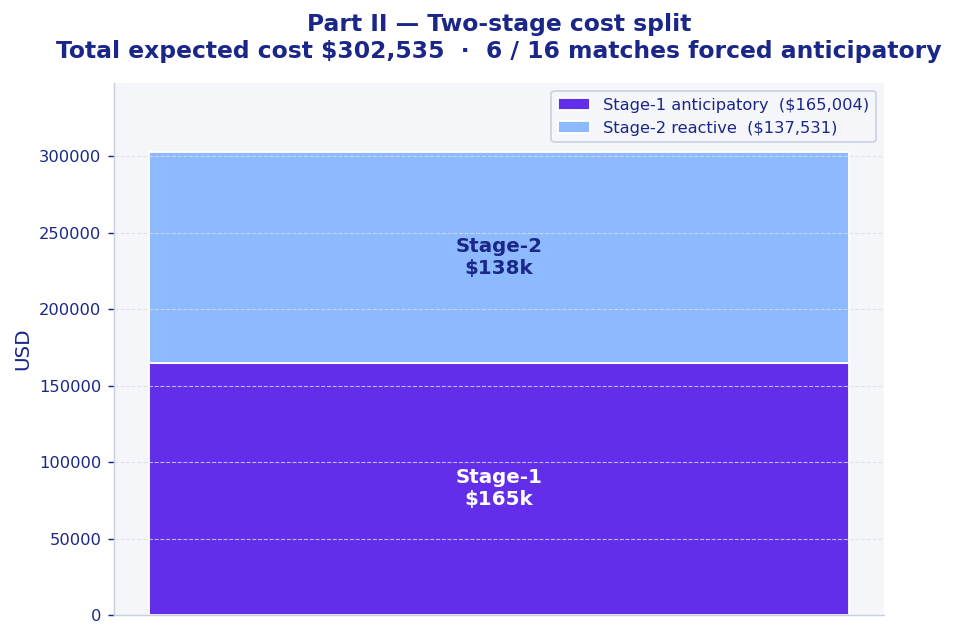
\includegraphics[width=0.55\textwidth]{part2_stage_split.png}
\caption{Two-stage cost split. Stage-1 anticipatory (purple, \USD{165k}) plus Stage-2 expected reactive (light blue, \USD{138k}) yields a total expected cost of \USD{303k}.}
\label{fig:stage-split}
\end{figure}

\paragraph{Forced-anticipatory matches.} \Cref{fig:feasibility} compares each match's window (green) to its minimum transit time from the best available production site (red). When red plus the 1-day production lead time exceeds green, the match cannot be served reactively. Six matches meet this criterion: Match 73 (Los Angeles, day +1), Match 74 (Boston), Match 75 (Monterrey), Match 76 (Houston), Match 78 (Dallas), and Match 79 (Mexico City). \Cref{fig:forced-map} maps these venues geographically.

\begin{figure}[H]
\centering
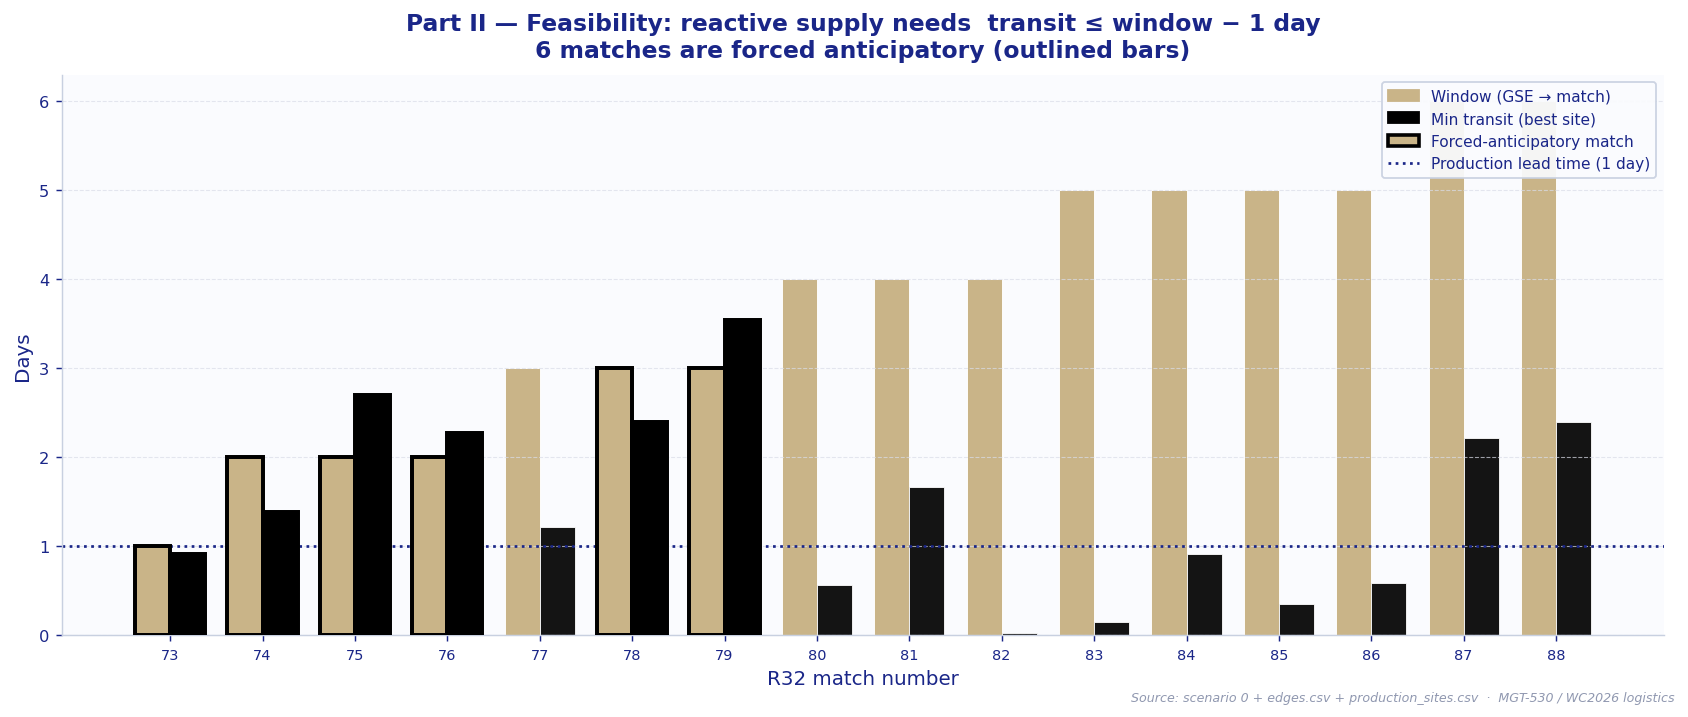
\includegraphics[width=\textwidth]{part2_feasibility.png}
\caption{Feasibility per R32 match. Green bars: time window from group-stage end (27 Jun) to match date. Red bars: minimum transit from any production site to the venue. Red-outlined bars are the 6 matches where transit + 1 day exceeds the window.}
\label{fig:feasibility}
\end{figure}

\begin{figure}[H]
\centering
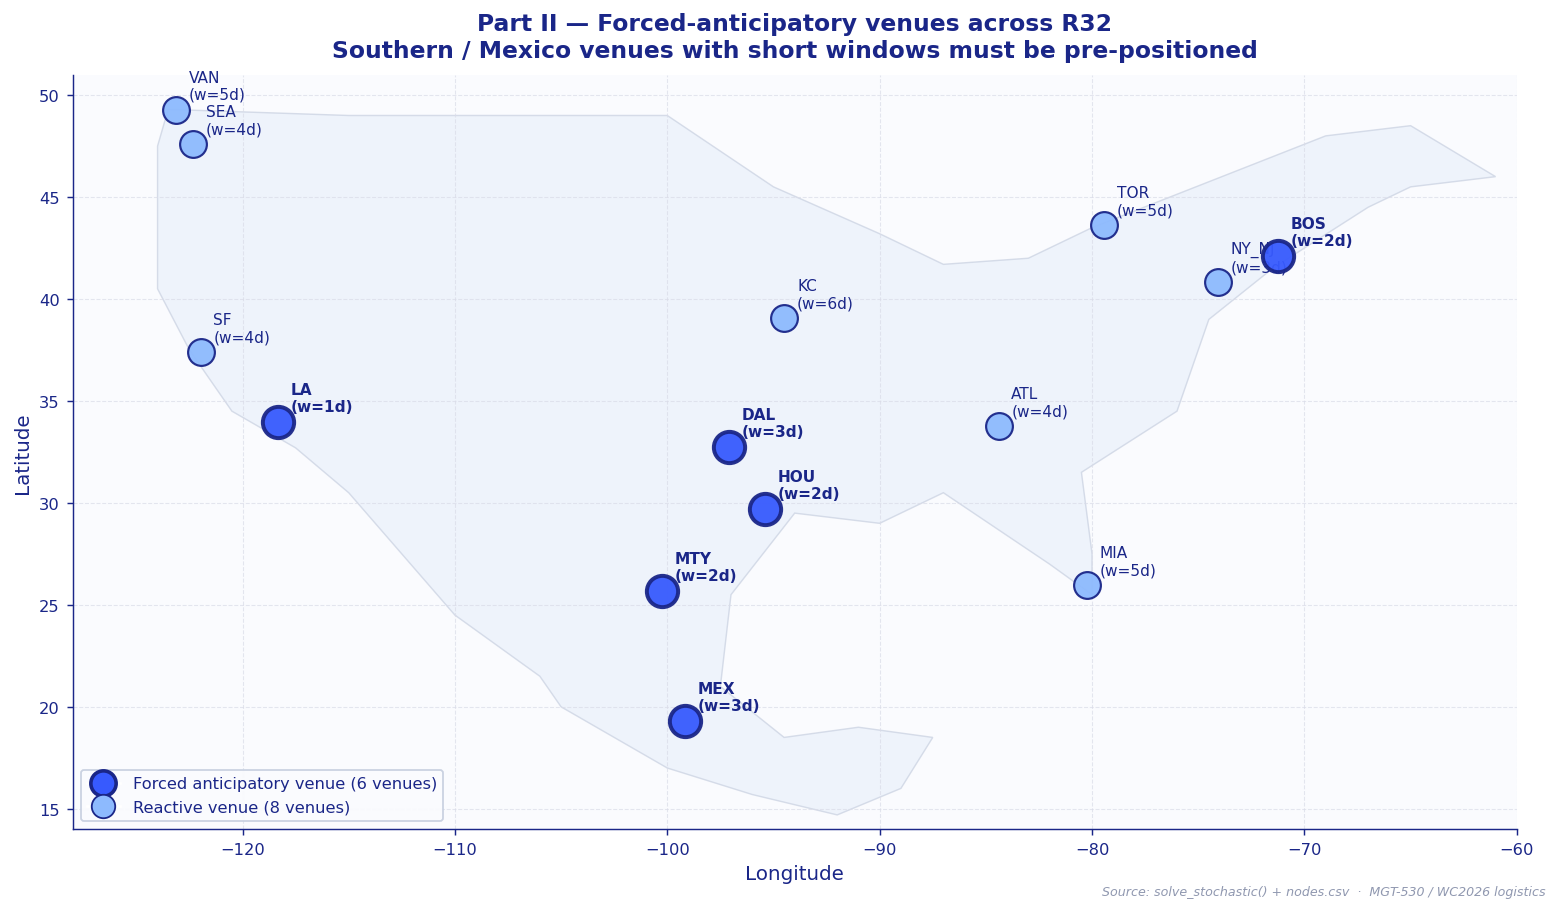
\includegraphics[width=0.95\textwidth]{part2_forced_map.png}
\caption{Spatial distribution of R32 venues. Red markers (6 venues) are forced anticipatory; lime markers (8 venues, some hosting two R32 matches) admit reactive supply. Forced venues cluster in the South and in Mexico.}
\label{fig:forced-map}
\end{figure}

\subsection{Sensitivity analysis}\label{sec:partII:sensitivity}

We probed four parameters: production cost (\USD{20}/\USD{50}/\USD{86} per~\msq), anticipatory waste factor (1$\times$/2$\times$/3$\times$), production lead time (0 or 1 day), and storage scenario (low/base/high). \Cref{fig:partII-tornado} ranks them by impact magnitude.

\begin{figure}[H]
\centering
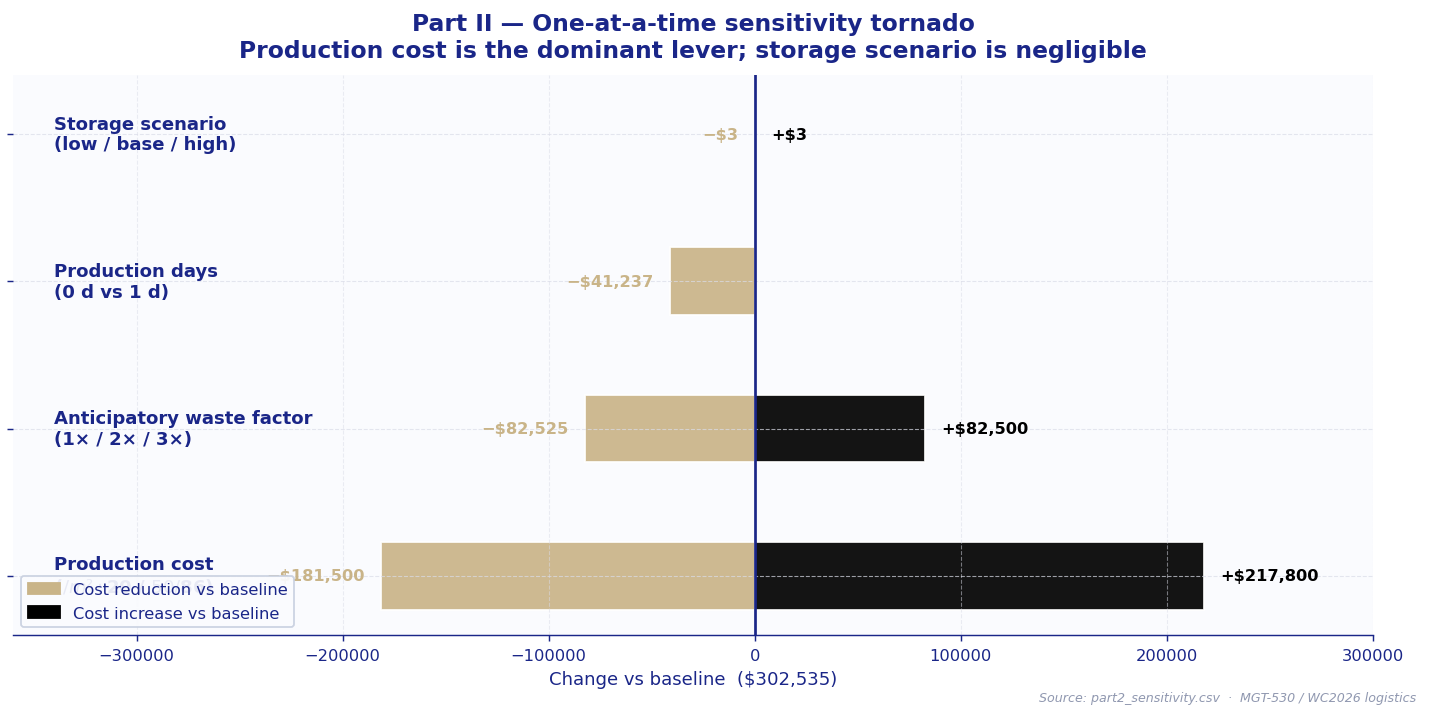
\includegraphics[width=\textwidth]{part2_sensitivity_tornado.png}
\caption{Part~II sensitivity tornado. Production cost dominates; the storage scenario is virtually invisible.}
\label{fig:partII-tornado}
\end{figure}

\paragraph{Production cost is the dominant driver.} \Cref{fig:prodcost} shows the linear cost response: every additional \USD{1}/\msq{} of production cost shifts the total expected cost by roughly \USD{6{,}000}.

\begin{figure}[H]
\centering
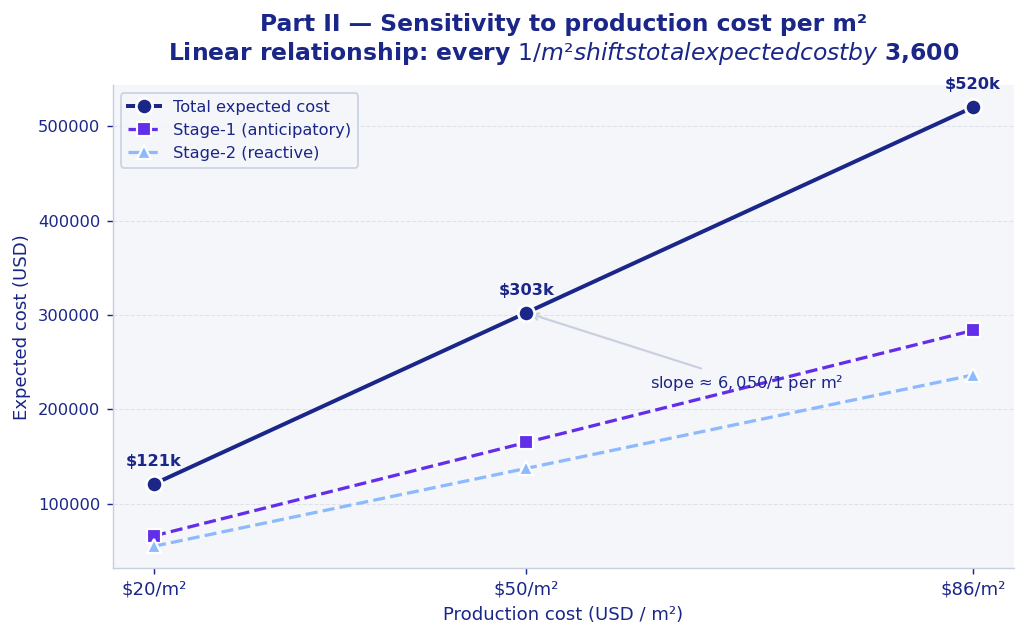
\includegraphics[width=0.85\textwidth]{part2_prod_cost_curve.png}
\caption{Sensitivity to production cost per \msq. The total response is linear; Stage-1 (with waste) has a steeper slope than Stage-2.}
\label{fig:prodcost}
\end{figure}

\paragraph{Same-day production halves forced matches.} The lead-time sweep is more interesting than the price sweep because it changes the \emph{structure} of the optimum. With $\mathrm{pd} = 0$ days, only 3 matches remain forced anticipatory (versus 6 at $\mathrm{pd} = 1$). The cost composition shifts dramatically: Stage-1 drops from \USD{165k} to \USD{83k} while Stage-2 rises from \USD{138k} to \USD{179k} — net total expected cost drops from \USD{303k} to \USD{261k}. Same-day production is therefore a structural lever, not just a cost lever.

\begin{figure}[H]
\centering
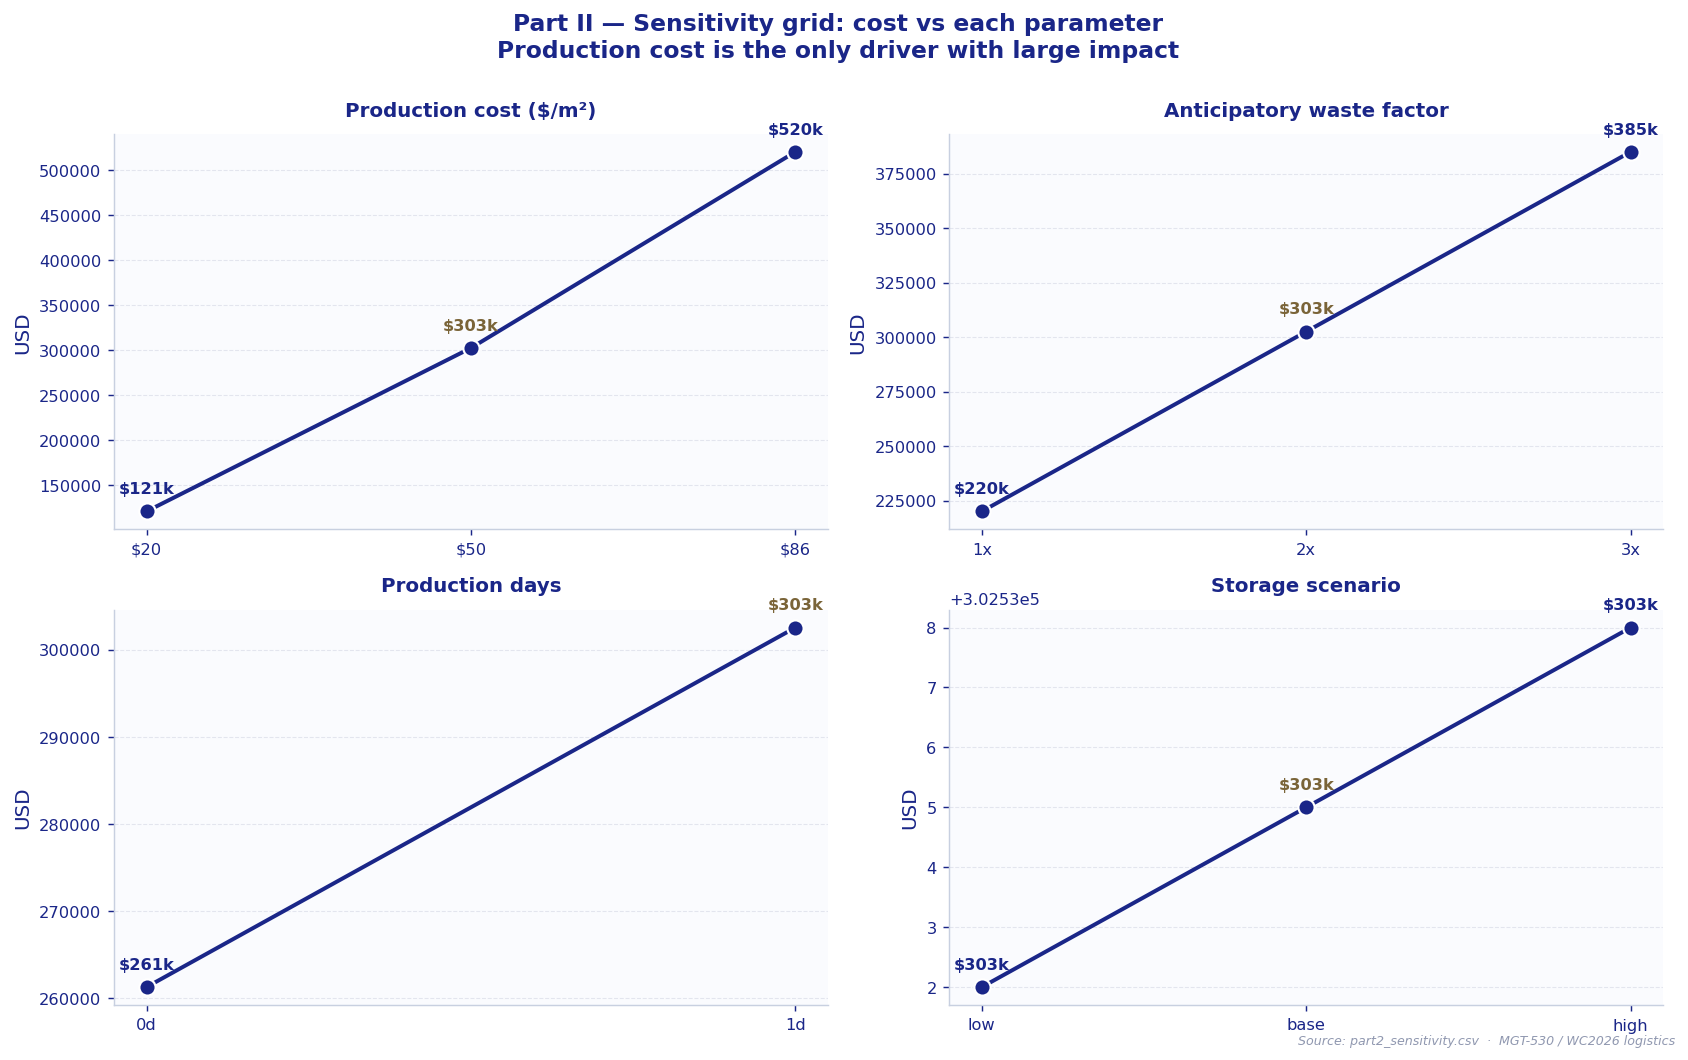
\includegraphics[width=\textwidth]{part2_sensitivity_grid.png}
\caption{Full sensitivity grid. Production cost and anticipatory waste produce material changes; storage is essentially flat; production days shifts costs between stages.}
\label{fig:sens-grid}
\end{figure}

\Cref{tab:partII-sens} reproduces the underlying sensitivity sweep.

\begin{table}[h]
\centering
\small
\caption{Part~II OAT sensitivity sweep.}
\label{tab:partII-sens}
\begin{tabular}{@{}llrrrl@{}}
\toprule
\textbf{Parameter} & \textbf{Value} & \textbf{Total} & \textbf{Stage-1} & \textbf{Stage-2} & \textbf{Forced} \\
\midrule
production cost   & \$20/m\textsuperscript{2}  & \USD{121{,}035} & \USD{66{,}004}  & \USD{55{,}031}  & 6 \\
production cost   & \$50/m\textsuperscript{2}  & \USD{302{,}535} & \USD{165{,}004} & \USD{137{,}531} & 6 \\
production cost   & \$86/m\textsuperscript{2}  & \USD{520{,}335} & \USD{283{,}804} & \USD{236{,}531} & 6 \\
anticipatory waste & 1$\times$                 & \USD{220{,}010} & \USD{192{,}509} & \USD{27{,}501}  & 6 \\
anticipatory waste & 2$\times$                 & \USD{302{,}535} & \USD{165{,}004} & \USD{137{,}531} & 6 \\
anticipatory waste & 3$\times$                 & \USD{385{,}035} & \USD{247{,}504} & \USD{137{,}531} & 6 \\
production days    & 0 (same-day)              & \USD{261{,}298} & \USD{82{,}502}  & \USD{178{,}796} & \textbf{3} \\
production days    & 1 (rush)                  & \USD{302{,}535} & \USD{165{,}004} & \USD{137{,}531} & 6 \\
storage scenario   & low                       & \USD{302{,}532} & \USD{165{,}001} & \USD{137{,}531} & 6 \\
storage scenario   & base                      & \USD{302{,}535} & \USD{165{,}004} & \USD{137{,}531} & 6 \\
storage scenario   & high                      & \USD{302{,}538} & \USD{165{,}007} & \USD{137{,}531} & 6 \\
\bottomrule
\end{tabular}
\end{table}

%==============================================================================
%  SECTION 5 — MANAGERIAL INSIGHTS AND RECOMMENDATIONS
%==============================================================================
\section{Managerial insights and recommendations}\label{sec:recommendations}

The two models together yield three actionable recommendations. Each is anchored in a quantitative result and supported by a sensitivity check.

\subsection{R1 --- Treat LED as a separate, weight-driven, FCL-only stream}

The dominant driver of Part~I container count is the 26-tonne FEU weight ceiling acting on the dense LED material (Section~\ref{sec:partI:setup}). Counting only volume would understate the FEU count by 44\%: 40 vs 71 containers. \Cref{fig:feu-eff} captures this in one image — 100\% volume fill of LED would weigh 256\% of the allowance.

\paragraph{Recommendation.} Procurement decisions for LED must use weight, not volume, as the binding constraint. Two operational consequences follow:
\begin{enumerate}[leftmargin=*,itemsep=2pt,topsep=2pt]
\item Maintain a separate LED FEU contract distinct from soft-goods FCL/LCL flows; do not allow mixed loading.
\item Investigate local LED rental in North America where contractually feasible. Even a 50\% local-rental share would remove $\sim$21 maritime FEUs and a corresponding share of the \USD{310k} ocean-freight bill, with a proportional reduction in Scope-3 CO\textsubscript{2} emissions.
\end{enumerate}

\subsection{R2 --- Two hubs (West + East) are sufficient; depot location is determined by port location}

The optimal solution opens exactly two depots (LAX and EWR), each co-located with the largest port on its side of the continent. The flow matrix in \Cref{fig:flow-mat} shows a clean West/East split with only Kansas City split between depots. Adding a third depot (Dallas, Miami, or Toronto candidates) does not improve cost: the additional fixed cost outweighs the trucking saving.

\paragraph{Recommendation.} The model demonstrates that depot location is essentially \emph{co-determined} by port choice — the depots cluster on the ports. Practical implication: negotiate a single integrated port-plus-depot contract per coast (West + East), rather than separating port and depot procurement.

\subsection{R3 --- Pre-position kits for short-window venues; invest in same-day production capability}

The 6 forced-anticipatory R32 matches concentrate at the Mexican venues (Monterrey, Mexico City) and at Houston, Dallas, Boston, and Los Angeles' day-after-group-stage opener. Their windows of 1--3 days are simply too short for reactive supply from any current production site (\Cref{fig:feasibility}). Going to a same-day production lead time (0 days) reduces the forced set from 6 matches to 3.

\paragraph{Recommendation.} Two complementary actions:
\begin{enumerate}[leftmargin=*,itemsep=2pt,topsep=2pt]
\item For the 6 forced-anticipatory matches, pre-print and pre-position candidate-team flag kits (typically 2--3 likely opponents) at the venue $\sim$2 weeks in advance, accepting the $2\times$ waste factor as the cost of certainty.
\item Invest in same-day large-format printing capability at the southernmost U.S. production sites (Tampa, the Carolinas). Under current parameters, this would shift \USD{83k} from Stage-1 anticipatory to a smaller Stage-2 reactive bill, net-saving \USD{41k} and halving the forced-anticipatory set.
\end{enumerate}

\subsection{Sustainability lens}

Ocean freight is 68\% of the Part~I cost, and ocean freight is also the dominant Scope-3 contributor in branding logistics. Any reduction in maritime FEU count — whether through local LED rental (R1), demand reduction, or load-rate improvements — has a proportionate emissions benefit. The anticipatory waste factor in Part~II ($2\times$) is a small but real source of physical material waste; reducing it through smarter candidate-team forecasting (R3) is the sustainability-aware analogue of R3.

%==============================================================================
%  SECTION 6 — LIMITATIONS
%==============================================================================
\section{Limitations and future work}\label{sec:limitations}

\paragraph{Storage costs are assumed.} FIFA's depot storage cost is not publicly available. We adopt a low/base/high sensitivity range (\USD{0.03}, \USD{0.08}, \USD{0.15} per~\mcube/day) and demonstrate that within this range the optimal solution is essentially invariant (\Cref{tab:partII-sens}). A real implementation would replace this assumption with negotiated contract values.

\paragraph{LED treated as imported.} The model assumes all LED is shipped from China — an explicit upper bound rationalised in Section~\ref{sec:partI} as a worst case. Local LED rental, where feasible, would halve the maritime FEU count and shift the cost profile dramatically. This is the single most attractive structural extension and a candidate for follow-up modelling.

\paragraph{Single-period model.} Both parts collapse the tournament into a single decision epoch. A multi-period model could capture phased deliveries (group-stage materials shipped earlier than knock-out materials), staged depot openings, and inventory roll-over. The complexity gain is modest but the modelling effort is non-trivial.

\paragraph{Stochastic scope limited to R32.} Part~II addresses only the Round of 32 (the round with the largest uncertainty). Quarter-finals onwards are simpler because demand collapses to the same eight remaining teams in increasingly known structure. An extension would add a multi-stage stochastic program coupling R32, R16, QF, SF, and Final.

\paragraph{Emissions are implicit.} We use cost as a proxy for environmental impact (cost-driven choices coincide with mode-shift and load-factor improvements). A first-class extension would replace the cost objective with a multi-objective cost / CO\textsubscript{2} formulation, using container-class-specific emission factors per~\mcube/km.

\paragraph{Single-objective deterministic equivalent.} The Part~II program minimises \emph{expected} total cost; a risk-averse decision-maker would prefer a CVaR or robust-optimisation formulation that protects against the worst $\alpha\%$ of scenarios. With only 50 scenarios this is a one-day modelling extension.

\paragraph{Plackett-Luce strengths are odds-derived.} Our team-strength prior (Equation~\ref{eq:strength}) comes from tournament-winner odds, which capture overall strength but not the round-by-round profile (e.g., a team strong in knock-out football but weak in groups). A richer prior could use round-specific qualification odds from the same bookmakers, or Elo-based ratings.

%==============================================================================
%  SECTION 7 — CONCLUSION
%==============================================================================
\section{Conclusion}\label{sec:conclusion}

This report formulates and solves two complementary optimisation models for the venue-branding logistics of FIFA World Cup 2026. Part~I, a multidimensional Location-Routing Problem on 16 stadiums, 5 ports and 7 candidate depots, yields a \USD{458{,}626} / 71-FEU optimal generic-branding flow through three open ports (LA, NY, VAN) and two open depots (LAX, EWR). The model's distinguishing feature — a multidimensional FEU constraint binding both volume and weight — produces a 44\% FEU surcharge for LED material that volume-only formulations would miss entirely. Part~II, a two-stage stochastic MILP over 50 Plackett-Luce-generated R32 scenarios, identifies 6 of 16 matches whose time windows preclude reactive supply and must be served by pre-positioned anticipatory material. Total expected cost is \USD{302{,}535}, of which Stage-1 anticipatory commitment accounts for \USD{165k}.

The split between the two parts mirrors the underlying physics: 99.8\% of the volume is generic and cost-driven; 0.2\% is nominative and time-driven under uncertainty. The recommendations follow this structure — separate LED procurement under weight constraints (R1), consolidate the network in two coastal hubs (R2), and invest in pre-positioning plus same-day production capability for the southernmost venues (R3).

All results are reproducible end-to-end via the commands documented in the project README at \url{https://github.com/rayangannoun-png/wc2026_logistics}. The Python implementation uses Google's OR-Tools \cite{ortools} as the modelling layer and SCIP \cite{scip} as the solver back-end; both models solve in well under one second.

%==============================================================================
%  REFERENCES
%==============================================================================
\printbibliography[heading=bibnumbered]

%==============================================================================
%  APPENDICES
%==============================================================================
\appendix

\renewcommand{\thesection}{\Alph{section}}
\renewcommand{\thefigure}{\Alph{section}.\arabic{figure}}
\renewcommand{\thetable}{\Alph{section}.\arabic{table}}

\titleformat{\section}
  {\color{NavyFIFA}\Large\bfseries\sffamily}{Appendix \thesection.}{0.7em}{}

%------------------------------------------------------------------------------
\section{Inventory reconstruction methodology (Qatar 2022 \texorpdfstring{$\to$}{->} WC2026)}\label{app:reconstruction}
\setcounter{figure}{0}
\setcounter{table}{0}

This appendix details the demand reconstruction summarised in Section~\ref{sec:data:demand}.

\subsection*{A.1 Three-tier confidence framework (Qatar 2022)}

The Qatar 2022 reconstruction starts from The Look Company's published total of $\sim$905{,}000~\msq{} \cite{thelookcompany_qatar}, of which we retain $\sim$640{,}000~\msq{} as the relevant ``stadium + immediate precinct'' scope (excluding city dressing and non-competition venues). \Cref{tab:tiers} reports the three-tier confidence classification.

\begin{table}[h]
\centering
\small
\caption{Qatar 2022 demand decomposition by confidence tier.}
\label{tab:tiers}
\begin{tabularx}{\textwidth}{@{}l X r@{}}
\toprule
\textbf{Tier} & \textbf{Postes} & \textbf{Approx. \msq{}} \\
\midrule
T1 — directly calculable & fence scrim (60 km, 2 m height), wayfinding totems (700 units), 151 vehicle wraps & 130{,}000 \\
T2 — adapted benchmarks  & building wraps (8 stadiums $\times$ 9{,}300~\msq{}), seat covers (8 $\times$ 3{,}000~\msq{}), pitch-side imprint & 104{,}000 \\
T3 — residual (interior) & concourses, tunnels, suites, vomitoires, decals, interior wayfinding (gap-fill) & 406{,}000 \\
\midrule
\textbf{Total Qatar 2022 (retained scope)} & & \textbf{640{,}000} \\
\bottomrule
\end{tabularx}
\end{table}

\subsection*{A.2 Volumetric conversion (anchored rouleau methodology)}

We convert \msq{} to \mcube{} using a physical anchor: standard ARC 14mil PVC mesh roll (60'' $\times$ 150') \cite{arcsupplies_rolls}, dimensioned at 1.52~m $\times$ 45.7~m = 69.5~\msq{} of material packed in a cylinder of $\varnothing$~0.18~m $\times$ 1.55~m = 0.039~\mcube{}, yielding a packed-roll density of $0.039/69.5 = 5.6\times 10^{-4}$~\mcube/\msq.

Cylindrical rolls do not interlock perfectly inside a container; industry practice estimates the realistic fill rate at $0.57$ (i.e., 43\% void). The effective volumetric conversion is therefore:
\[
V_{\text{container}}\ (\mcube)\ =\ A\ (\msq) \times \frac{5.6 \times 10^{-4}}{0.57}\ \approx\ A \times 9.83 \times 10^{-4}.
\]

\subsection*{A.3 WC2026 extrapolation (three scaling factors)}

Three factors transform Qatar 2022 into WC2026:
\begin{enumerate}[leftmargin=*,itemsep=2pt,topsep=2pt]
\item \textbf{Capacity factor} ($\times 2$): 8 $\to$ 16 stadiums, with average capacity larger ($+15$\%).
\item \textbf{Fixed-scope neutrality}: city dressing remains out-of-scope (as in Qatar).
\item \textbf{Typology disruption}: a new ``brand scrubbing'' poste (masking NFL/club logos) appears, contributing an additional $\sim$69{,}000~\msq{}.
\end{enumerate}
The resulting WC2026 totals are 1{,}480{,}000~\msq{} and 2{,}726~\mcube. \Cref{tab:wc2026-demand} reports the poste-level demand breakdown.

\begin{table}[h]
\centering
\small
\caption{WC2026 demand by poste (totals across 16 stadiums).}
\label{tab:wc2026-demand}
\begin{tabular}{@{}lrrrl@{}}
\toprule
\textbf{Poste} & \textbf{Volume (\mcube)} & \textbf{Weight (\tonne)} & \textbf{Class} & \textbf{Key} \\
\midrule
LED perimeter   & 1{,}072 & 1{,}066 & LED  & fixed (1 per stadium) \\
Interior        &   912   &   464   & SOFT & capacity \\
Fence scrim     &   236   &    43   & SOFT & fixed (precinct perimeter) \\
Building wraps  &   160   &   109   & SOFT & capacity \\
Totems (alu)    &   140   &    56   & SOFT & fixed (per stadium) \\
Brand scrubbing &    68   &    35   & SOFT & typology (3 tiers) \\
Masts           &    60   &    24   & SOFT & fixed (per stadium) \\
Seat covers     &    54   &    17   & SOFT & capacity \\
Pitch-side      &    11   &     7   & SOFT & fixed (pitch perimeter) \\
Vehicle wraps   &     7   &     5   & SOFT & capacity \\
Wayfinding      &     6   &     2   & SOFT & fixed \\
\midrule
\textbf{Total}  & \textbf{2{,}726} & \textbf{1{,}828} & --- & --- \\
\bottomrule
\end{tabular}
\end{table}

\subsection*{A.4 Brand scrubbing — the 2026-specific poste}

Brand scrubbing reflects the FIFA contractual obligation to mask all pre-existing commercial branding on host venues \cite{themirror_scrubbing}. The anchor is a journalistically-reported figure of $\sim$2{,}000 brand elements at Mercedes-Benz Stadium (Atlanta) \cite{sbj_facilitiesdive}. We assume an average of 3~\msq{} per masked element (range 0.5--10~\msq{} depending on logo size), and segment the 16 venues into three tiers:
\begin{itemize}[leftmargin=*,itemsep=2pt,topsep=2pt]
\item 8 heavily-branded NFL venues: $\sim$2{,}000 elements $\times$ 3~\msq{} = 6{,}000~\msq{} per venue;
\item 5 recent venues with lighter branding: $\sim$1{,}000 elements $\times$ 3~\msq{} = 3{,}000~\msq{} per venue;
\item 3 Mexican/Canadian venues with minimal pre-existing branding: $\sim$700 elements $\times$ 3~\msq{} = 2{,}100~\msq{} per venue.
\end{itemize}
The total of 69{,}000~\msq{} carries the largest single uncertainty in the reconstruction; a sensitivity range of 40{,}000--100{,}000~\msq{} is defensible.

\subsection*{A.5 Per-stadium demand heatmap}

\Cref{fig:heatmap} visualises the full per-stadium, per-poste demand matrix.

\begin{figure}[H]
\centering
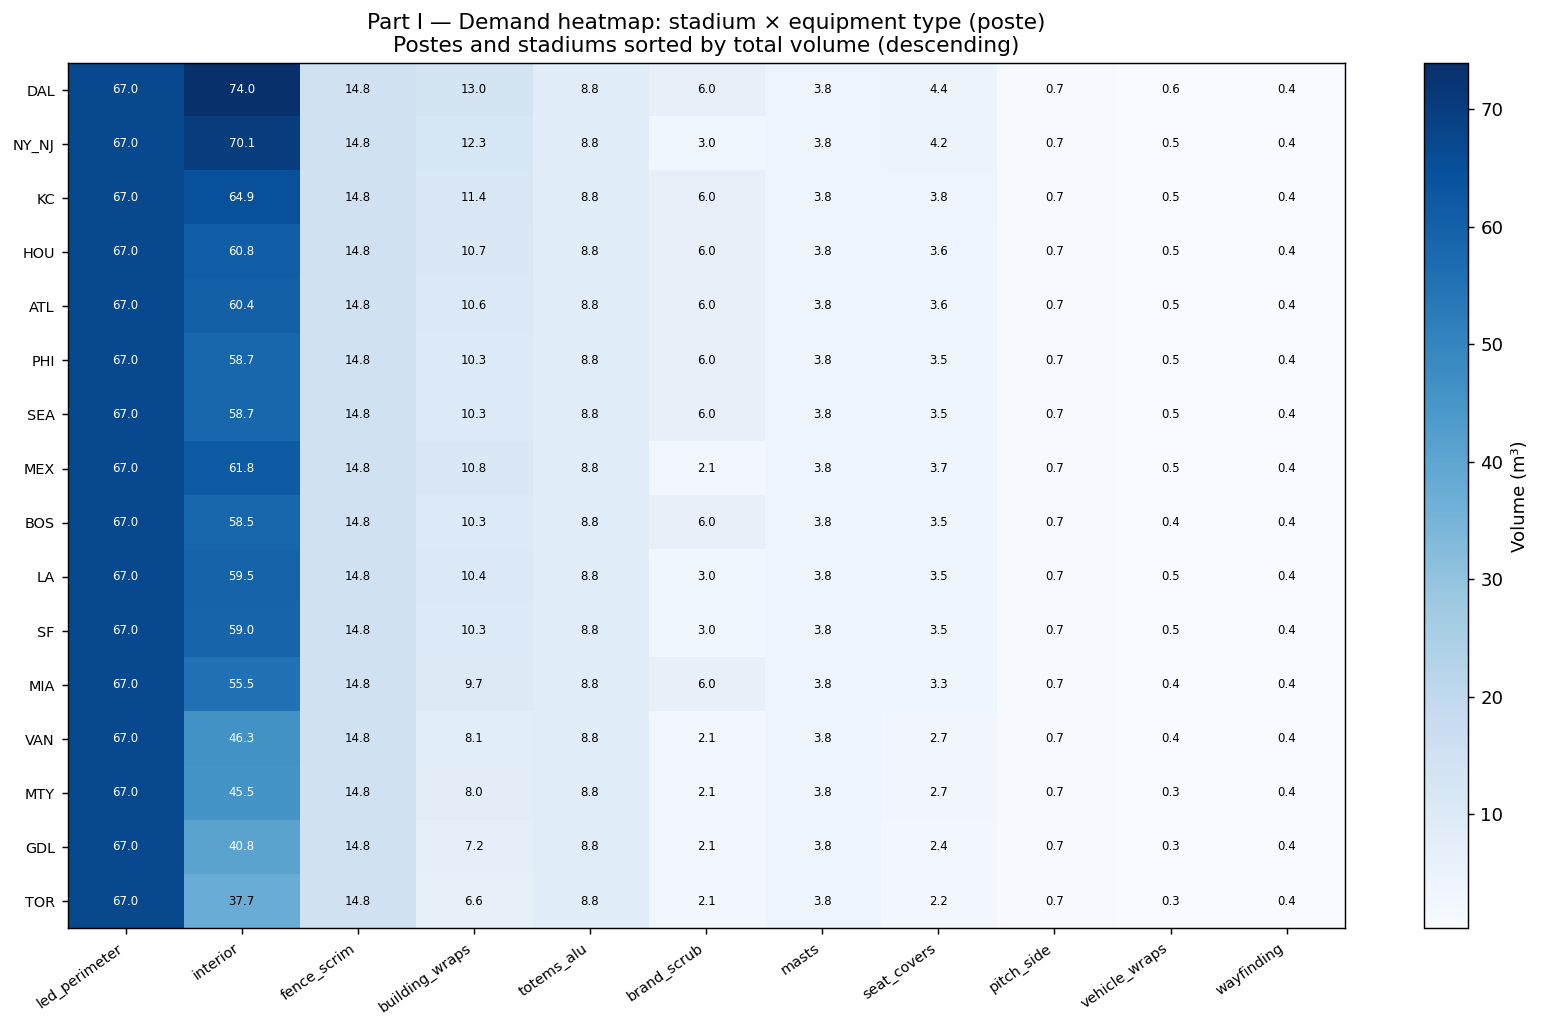
\includegraphics[width=\textwidth]{part1_demand_heatmap.png}
\caption{Full demand heatmap. Stadiums (rows) and postes (columns), sorted by total volume.}
\label{fig:heatmap}
\end{figure}

%------------------------------------------------------------------------------
\section{Full assumptions registry}\label{app:assumptions}
\setcounter{figure}{0}
\setcounter{table}{0}

\Cref{tab:assumptions} catalogues all 20 assumptions in the project, classified as: \statusSourced{} externally sourced, \statusDerived{} derived from project data, or \statusAssumed{} assumed-with-sensitivity.

\begin{longtable}{@{}p{0.36\textwidth}p{0.22\textwidth}c p{0.30\textwidth}@{}}
\caption{Full assumptions registry.\label{tab:assumptions}}\\
\toprule
\textbf{Assumption} & \textbf{Value} & \textbf{Status} & \textbf{Source / sensitivity}\\
\midrule
\endfirsthead
\toprule
\textbf{Assumption} & \textbf{Value} & \textbf{Status} & \textbf{Source / sensitivity}\\
\midrule
\endhead
\midrule
\multicolumn{4}{r}{\textit{continued on next page}}\\
\endfoot
\bottomrule
\endlastfoot
Container payload limit & 26~\tonne & \statusSourced{} & ISO gross 30.48~\tonne, U.S. road \cite{fmcsa_weight,iso_container} \\
Container interior volume & 67~\mcube & \statusSourced{} & ISO 40-ft standard \cite{iso_container} \\
Truck usable volume & 90~\mcube & \statusSourced{} & U.S. dry-van trailer 53~ft \\
Container fill rate & 0.57 & \statusDerived{} & Rouleau geometry + voids \cite{arcsupplies_rolls} \\
LED density & 0.99~\tonne/\mcube & \statusDerived{} & 1{,}066~\tonne / 1{,}072~\mcube{} from inventory \\
Soft density & 0.46~\tonne/\mcube & \statusDerived{} & 762~\tonne / 1{,}654~\mcube{} from inventory \\
Production cost & \USD{50}/\msq & \statusSourced{} & U.S. large-format \cite{costhack_printing}; range \$20/\$50/\$86 \\
Rush production lead time & 1 day & \statusSourced{} & Industry \cite{signsnyc_rush}; sensitivity 0/1 day \\
Storage cost & \USD{0.03}/\USD{0.08}/\USD{0.15} \mcube/day & \statusAssumed{} & FIFA cost not public; low/base/high sensitivity \\
Anticipatory waste factor & 2$\times$ & \statusAssumed{} & 2 candidate teams; sensitivity 1$\times$/2$\times$/3$\times$ \\
Storage horizon & 30 days & \statusAssumed{} & Storage time before R32 \\
Nominative material per match & 275~\msq & \statusSourced{} & Inventory: flags 75 + decals 150 + backdrops 50 \\
Part~I storage excluded & --- & \statusDerived{} & Cat-1 transits, no long stock \\
LED routing direct port$\to$stadium & --- & \statusDerived{} & 1 system/stadium; oversized/fragile \cite{jyvisions_led} \\
Depot capacity uncapacitated & --- & \statusDerived{} & Capacity column empty in CSV (UFLP) \\
Origin: all from China + local print & --- & \statusDerived{} & Inventory assumption; raw imported, printed locally \\
Scenario count & 50, equiprobable & \statusAssumed{} & Monte-Carlo sample size \\
Demand ventilation & 3 keys (cap / fix / typ) & \statusDerived{} & Per-poste physics; reconciles to 2{,}726~\mcube \\
Team strengths from odds & --- & \statusSourced{} & Bookmaker odds, validated vs Opta \cite{opta_supercomputer} \\
Network costs (ports/depots/edges) & --- & \statusSourced{} & Project CSVs \\
\end{longtable}

%------------------------------------------------------------------------------
\section{Data dictionary}\label{app:datadict}
\setcounter{figure}{0}
\setcounter{table}{0}

\Cref{tab:csvs} lists every CSV in the data pipeline.

\begin{longtable}{@{}p{0.30\textwidth}r p{0.55\textwidth}@{}}
\caption{Data dictionary.\label{tab:csvs}}\\
\toprule
\textbf{File} & \textbf{Rows} & \textbf{Schema (columns)}\\
\midrule
\endfirsthead
\toprule
\textbf{File} & \textbf{Rows} & \textbf{Schema (columns)}\\
\midrule
\endhead
\bottomrule
\endlastfoot
\filename{data/raw/nodes.csv}            & 35  & node\_id, node\_name, city, region, country, node\_type (port/depot/stadium/site), latitude, longitude, confidence, status, notes \\
\filename{data/raw/ports.csv}            &  6  & node\_id, fcl\_rate\_feu\_usd, lcl\_rate\_m3\_usd, customs\_fixed\_cost\_usd, handling\_cost\_per\_feu\_usd, sea\_distance\_from\_china\_km \\
\filename{data/raw/depots.csv}           &  7  & node\_id, fixed\_setup\_cost\_usd, handling\_cost\_per\_m3\_usd, capacity\_proxy\_m3 (empty $\Rightarrow$ uncapacitated) \\
\filename{data/raw/stadiums.csv}         & 16  & node\_id, fifa\_name, common\_name, host\_city, metro\_area, country, venue\_cluster, capacity \\
\filename{data/raw/production\_sites.csv} & 6  & node\_id, provider (TLC / Wasserman), city, country, materials\_possible \\
\filename{data/raw/storage\_scenarios.csv} & 3 & scenario\_id (low/base/high), storage\_cost\_per\_m3\_day\_usd, basis \\
\filename{data/raw/edges.csv}             & 524 & origin\_node\_id, destination\_node\_id, edge\_type, mode (sea/road), distance\_km, transit\_time\_days, cost\_per\_km\_usd, border\_crossing, border\_cost\_usd \\
\filename{data/generated/stadium\_demand\_by\_poste.csv} & 176 & node\_id, stadium\_id, poste, class (led/soft), volume\_m3, weight\_t \\
\filename{data/generated/stadium\_demand\_by\_class.csv} & 16 & node\_id, stadium\_id, vol\_led\_m3, wt\_led\_t, vol\_soft\_m3, wt\_soft\_t, vol\_total\_m3, wt\_total\_t \\
\filename{data/generated/part2\_scenarios.csv} & 800 & scenario, probability, match, home\_team, away\_team, venue\_node, date \\
\end{longtable}

%------------------------------------------------------------------------------
\section{Detailed sensitivity results}\label{app:sensitivity}
\setcounter{figure}{0}
\setcounter{table}{0}

This appendix collects the supplementary sensitivity figures referenced in Sections~\ref{sec:partI:sensitivity} and~\ref{sec:partII:sensitivity}.

\begin{figure}[H]
\centering
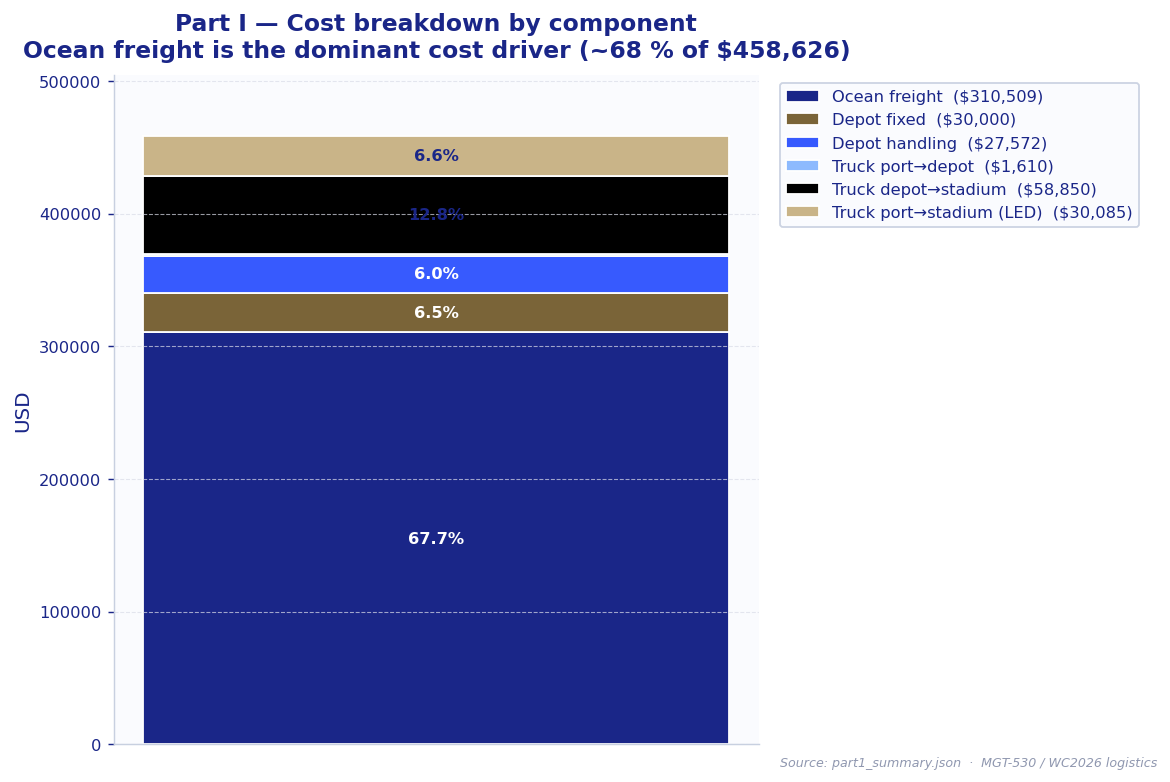
\includegraphics[width=\textwidth]{part1_cost_breakdown.png}
\caption{Part~I cost breakdown — stacked bar of the six cost components ($Z = \USD{458{,}626}$).}
\end{figure}

\begin{figure}[H]
\centering
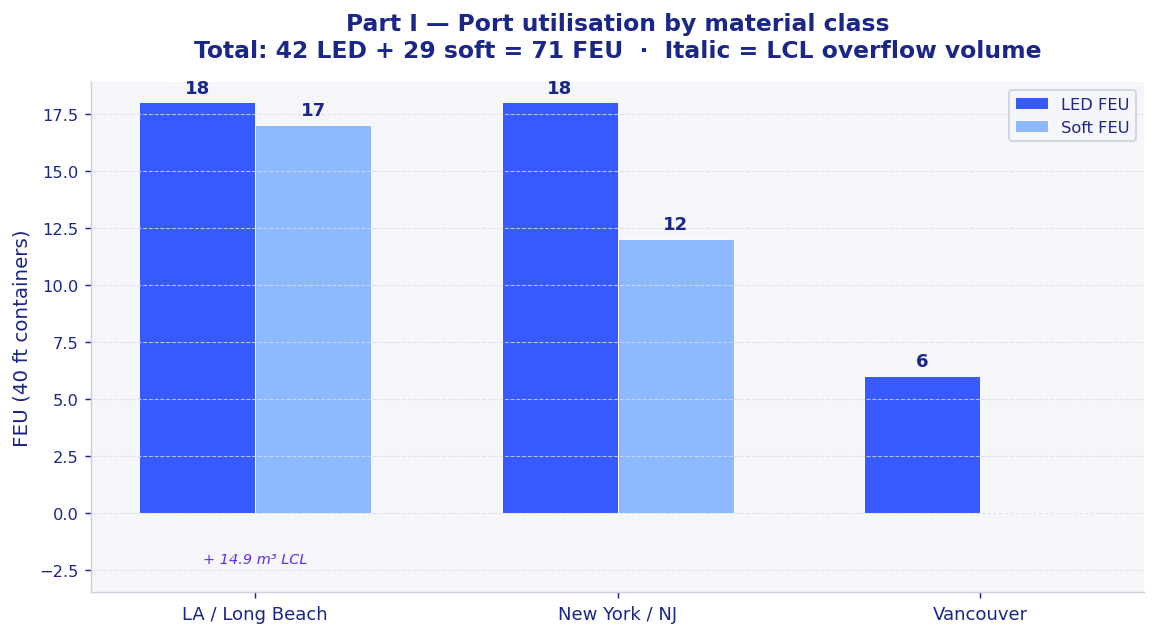
\includegraphics[width=0.85\textwidth]{part1_port_utilization.png}
\caption{Part~I port utilisation — FEU allocation by material class at each opened port. Vancouver carries only LED; LA shows the LCL overflow.}
\end{figure}

\begin{figure}[H]
\centering
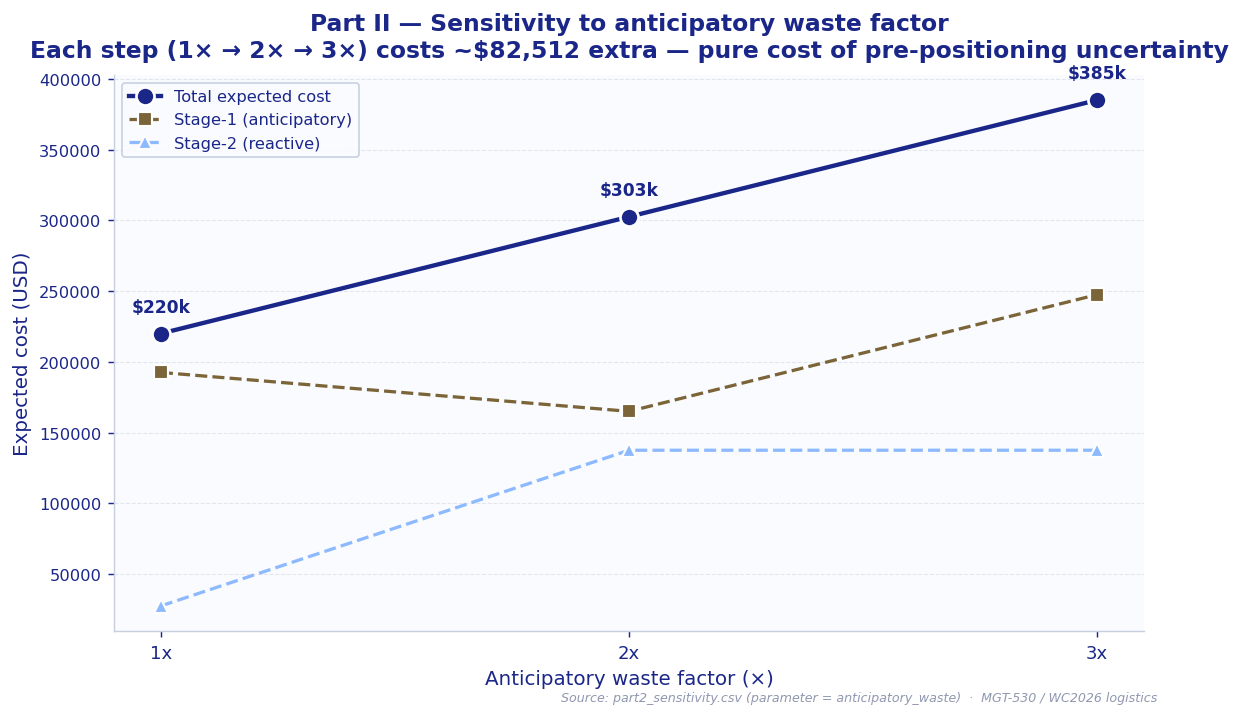
\includegraphics[width=\textwidth]{part2_waste_curve.png}
\caption{Part~II — anticipatory waste factor sensitivity. Each step (1$\times \to$ 2$\times \to$ 3$\times$) costs roughly \USD{82k} additional Stage-1 production.}
\end{figure}

\begin{figure}[H]
\centering
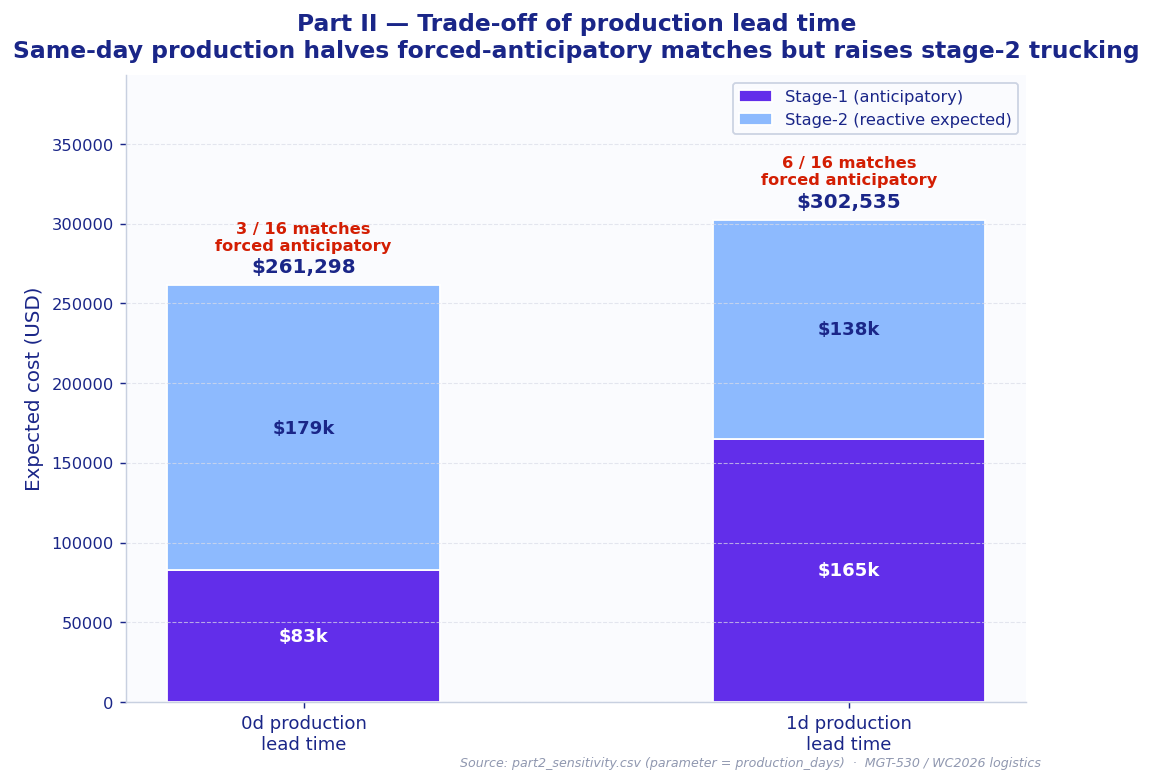
\includegraphics[width=0.85\textwidth]{part2_production_days.png}
\caption{Part~II — production lead time trade-off. Same-day production halves Stage-1 cost but raises Stage-2 expected cost; net total drops by \USD{41k}.}
\end{figure}

\begin{figure}[H]
\centering
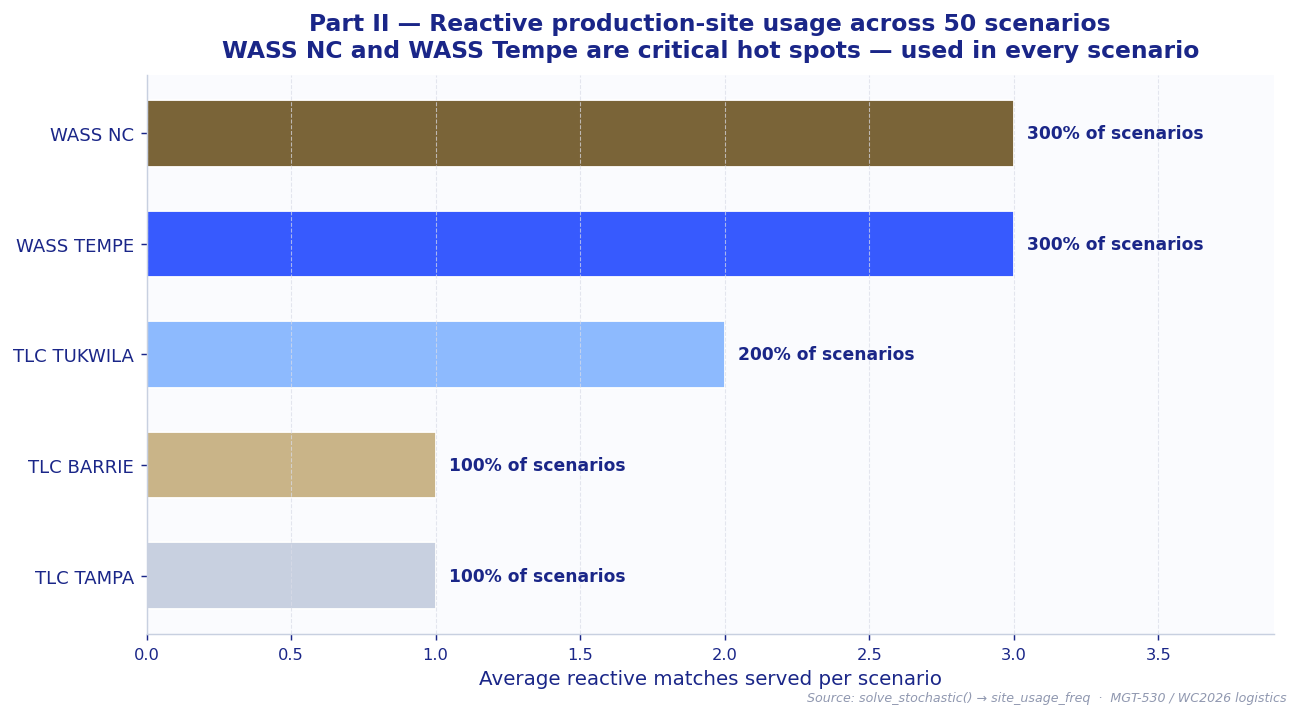
\includegraphics[width=\textwidth]{part2_reactive_sites.png}
\caption{Part~II reactive production-site usage across 50 scenarios. Wasserman North Carolina and Wasserman Tempe are the load-bearing facilities.}
\end{figure}

\begin{figure}[H]
\centering
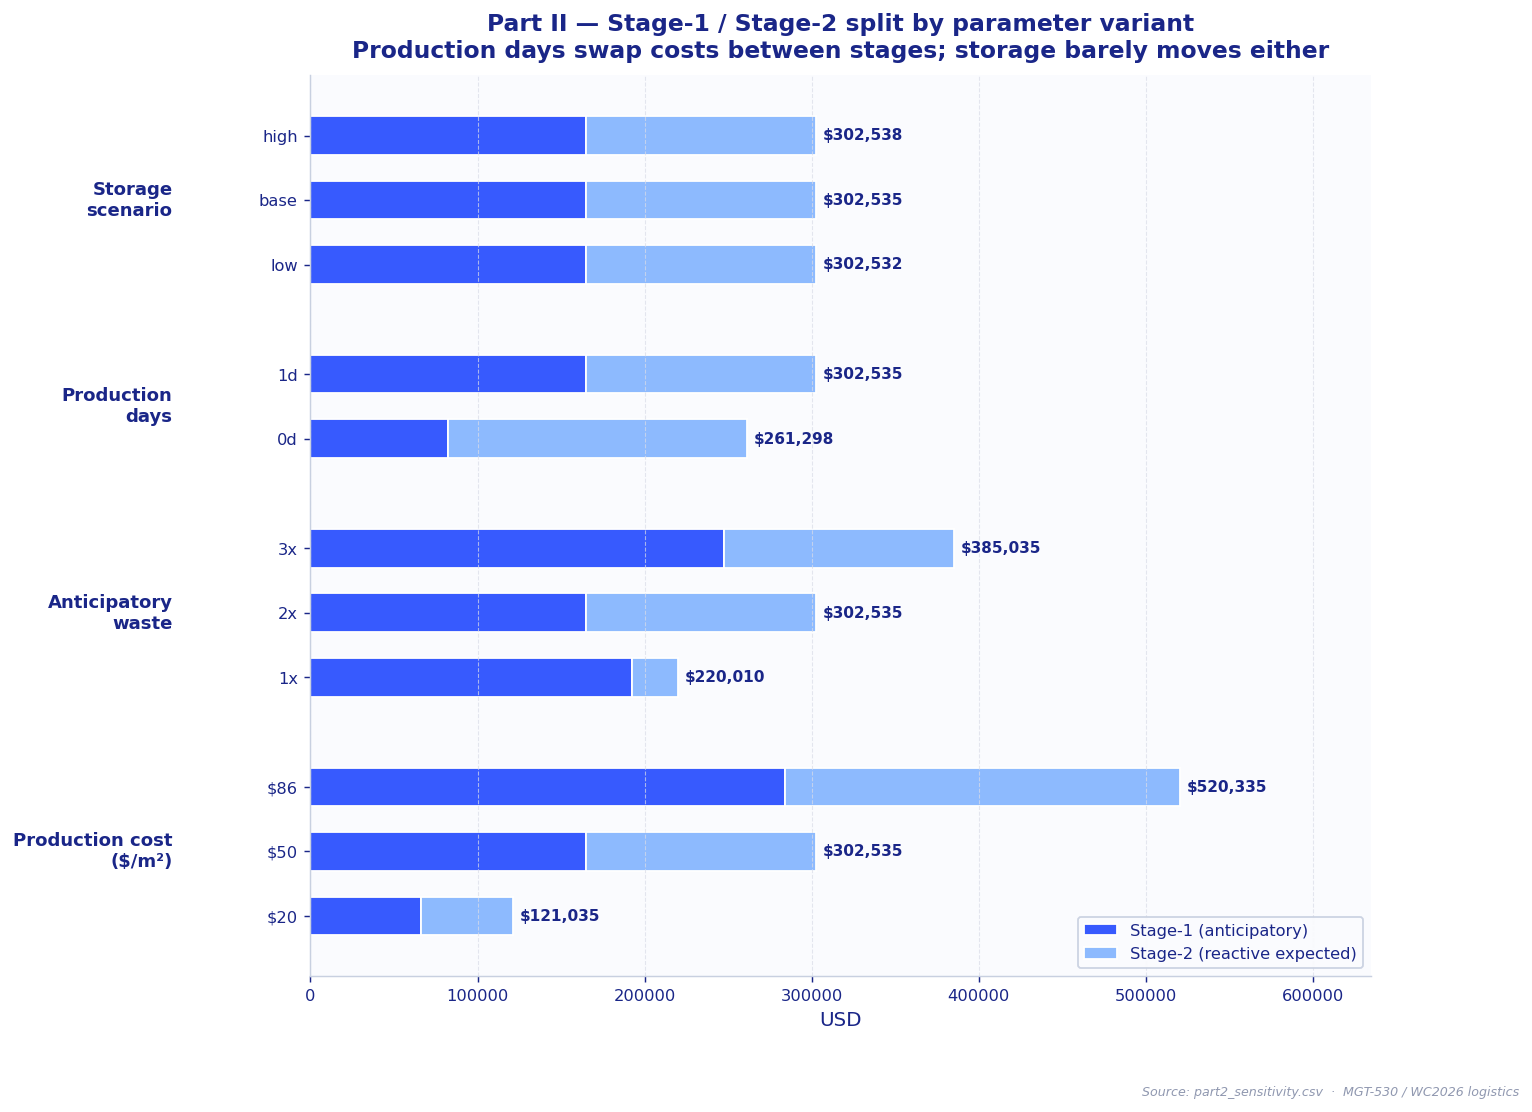
\includegraphics[width=\textwidth]{part2_stage_by_param.png}
\caption{Part~II Stage-1 vs Stage-2 cost by parameter variant. Production days shifts costs between stages; storage is essentially flat across variants.}
\end{figure}

\begin{figure}[H]
\centering
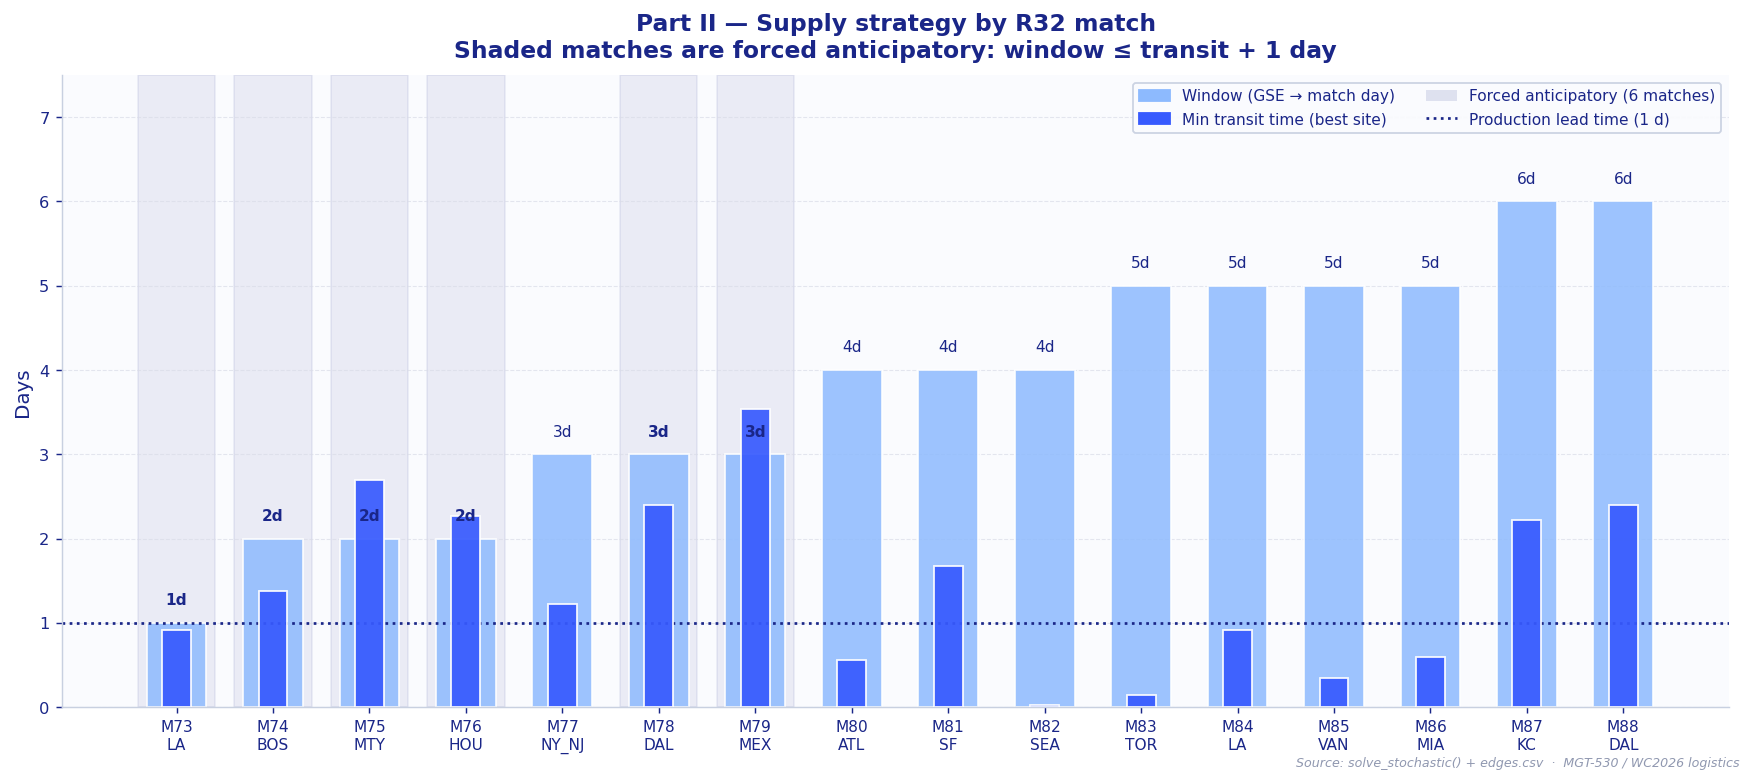
\includegraphics[width=\textwidth]{part2_anticipatory_by_match.png}
\caption{Part~II — anticipatory supply strategy per R32 match. Shaded matches are forced anticipatory; window length is annotated above each bar.}
\end{figure}

%------------------------------------------------------------------------------
\section{Categorised source registry}\label{app:sources}
\setcounter{figure}{0}
\setcounter{table}{0}

\Cref{tab:sources-cat} groups the sources by domain and notes the assumption(s) each justifies. The numbered references appear in the bibliography.

\begin{longtable}{@{}p{0.18\textwidth} p{0.50\textwidth} p{0.27\textwidth}@{}}
\caption{Source registry by category.\label{tab:sources-cat}}\\
\toprule
\textbf{Category} & \textbf{Source} & \textbf{Justifies}\\
\midrule
\endfirsthead
\toprule
\textbf{Category} & \textbf{Source} & \textbf{Justifies}\\
\midrule
\endhead
\bottomrule
\endlastfoot
Tournament       & FIFA 2026 official \cite{fifa2026official}            & Venues, schedule, format \\
                 & StadiumDB \cite{stadiumdb_wc2026}                      & Stadium capacities \\
                 & Wasserman Live \cite{wassermanlive_wc2026}             & 2026 service provider \\
Inventory        & The Look Company \cite{thelookcompany_qatar}           & Qatar 2022 baseline (905k~\msq) \\
                 & bluemedia Super Bowl \cite{bluemedia_superbowl}        & Building wrap ratio \\
                 & CSM Live \cite{csmlive_dressing}                       & Seat-cover ratio \\
                 & JYVISIONS \cite{jyvisions_led}                          & LED 1 FEU/stadium \\
                 & ARC Supplies \cite{arcsupplies_rolls}                  & Roll dimensions; rouleau anchor \\
                 & Camden Look \cite{camden_lookspec}                     & Material densities \\
                 & The Mirror / The Athletic \cite{themirror_scrubbing}   & FIFA clean-stadium clause \\
                 & SBJ / Facilities Dive \cite{sbj_facilitiesdive}        & Brand scrubbing element count \\
Logistics costs  & ISO 668 \cite{iso_container}                            & FEU dimensions \\
                 & FMCSA \cite{fmcsa_weight}                              & U.S. weight regulation \\
                 & Costhack \cite{costhack_printing}                       & Production cost \\
                 & Signs NYC \cite{signsnyc_rush}                          & Rush lead time \\
Methodology      & Daskin \cite{daskin_location}                          & LRP foundations \\
                 & Birge \& Louveaux \cite{birge_louveaux}                & Two-stage stochastic programming \\
                 & OR-Tools \cite{ortools}                                 & Modelling layer \\
                 & SCIP \cite{scip}                                        & MILP solver \\
                 & Plackett (1975) \cite{plackett1975}                    & Ranking model \\
                 & Opta supercomputer \cite{opta_supercomputer}            & Strength validation \\
                 & MGT-530 course material \cite{gallay_mgt530}           & Course-specific notation \\
\end{longtable}

%------------------------------------------------------------------------------
\section{Implementation and reproducibility}\label{app:reproducibility}
\setcounter{figure}{0}
\setcounter{table}{0}

\subsection*{Repository structure}
The project is hosted at \url{https://github.com/rayangannoun-png/wc2026_logistics}, with the following structure:
\begin{verbatim}
data/raw/          original project CSVs (network, ports, depots, edges)
data/generated/    data the team built (stadium demand, scenarios)
docs/              full decision log and model specifications
reference/         supporting documents (inventory reconstruction, course KB)
src/common/        data loader + visualisations + table export
src/part1_lrp/     deterministic LRP (model, demand builder, sensitivity)
src/part2_stochastic/  two-stage stochastic program (model, scenarios, sensitivity)
outputs/results/   solver outputs (CSV/JSON)
outputs/figures/   25 PNG figures (matplotlib)
\end{verbatim}

\subsection*{Reproducing all results}
\begin{verbatim}
pip install -r requirements.txt
python run_all.py     # 8 steps, ~30 s end-to-end on a laptop
\end{verbatim}
The pipeline (i) builds per-stadium demand, (ii) solves Part~I LRP, (iii) runs Part~I sensitivity, (iv) generates 50 R32 scenarios, (v) solves Part~II stochastic model, (vi) runs Part~II sensitivity, (vii) exports five result tables, (viii) generates all 25 figures.

\subsection*{Solver and tools}
The MILP models are formulated in Python using OR-Tools \cite{ortools} \code{pywraplp}, and solved with SCIP \cite{scip}. Both models solve to optimality in well under one second on a 2022-era laptop. Figures are produced with Matplotlib using the FIFA WC2026 brand palette throughout.

\subsection*{Software versions}
Python 3.11, OR-Tools 9.10, SCIP 8.1, Matplotlib 3.8, NumPy 1.26. Operating system: macOS 14 (Sonoma) and Linux Ubuntu 22.04 — both tested.

\subsection*{Team contributions}
The raw network CSVs (\filename{nodes.csv}, \filename{ports.csv}, \filename{depots.csv}, \filename{stadiums.csv}, \filename{production\_sites.csv}, \filename{edges.csv}) were compiled by a team member. The demand reconstruction, both optimisation models, the scenario generator, all 25 figures, all 11 result tables, and this report were produced by the author team listed on the cover page.

\end{document}
